\documentclass[12pt, a4paper]{article}

\usepackage{geometry}
\usepackage{tabularx}
\usepackage{booktabs}
\usepackage{hyperref}
\usepackage{titlesec}
\usepackage{enumitem}
\usepackage{tikz}
\usepackage{float}
\usepackage{needspace}
\usepackage{graphicx}
\usepackage{pdflscape}

\usepackage[utf8]{inputenc}
\usepackage[T5]{fontenc}
\usepackage[vietnamese]{babel}

\usepackage[table]{xcolor}
\geometry{a4paper, left=2.5cm, right=2.5cm, top=2.5cm, bottom=2.5cm}
\usetikzlibrary{arrows.meta, positioning, shapes.geometric}

\title{\textbf{Software Requirements Specification (SRS)}\\ Website Dự báo Xu hướng Giá Cổ phiếu Ngắn hạn bằng AI}
\author{Nhóm 5 - DKT}
\date{14/05/2026}

\setcounter{tocdepth}{3}
\setcounter{secnumdepth}{3}

\begin{document}

\maketitle
\thispagestyle{empty}

\noindent\textbf{Quản lý tài liệu (Document Control)}

\begin{table}[htbp]
    \centering
    \renewcommand{\arraystretch}{1.5}
    \begin{tabularx}{\textwidth}{|l|X|}
        \hline
        \rowcolor{cyan!15}
        \multicolumn{2}{|l|}{\textbf{Thông tin tài liệu}}                                                                \\
        \hline
        \textbf{Tiêu đề}             & Đặc tả yêu cầu phần mềm cho Website Dự báo Xu hướng Giá Cổ phiếu Ngắn hạn bằng AI \\
        \hline
        \textbf{Ngày tạo}            & 14/05/2026                                                                        \\
        \hline
        \textbf{Trạng thái}          & Bản thảo (Draft)                                                                  \\
        \hline
        \textbf{Phiên bản}           & 2.0                                                                               \\
        \hline
        \textbf{Đối tượng tiếp nhận} & Giảng viên Hướng dẫn, Hội đồng Đánh giá, Đội ngũ Phát triển                       \\
        \hline
        \textbf{Mã tài liệu}         & SRS\_AI\_STOCK\_PREDICT\_V2.0                                                     \\
        \hline
    \end{tabularx}
\end{table}

\noindent\textbf{Tuyên bố miễn trừ trách nhiệm (Disclaimer):}\\
Tài liệu này được cung cấp cho mục đích nghiên cứu học thuật. Nền tảng dự báo không đưa ra lời khuyên tài chính. Mọi quyết định đầu tư dựa trên dự báo của AI thuộc về trách nhiệm của người dùng.

\newpage
\tableofcontents
\newpage

\section*{Thuật ngữ và Định nghĩa (Glossary)}
\addcontentsline{toc}{section}{Thuật ngữ và Định nghĩa (Glossary)}

\begin{table}[htbp]
    \centering
    \renewcommand{\arraystretch}{1.5}
    \begin{tabularx}{\textwidth}{|l|X|}
        \hline
        \rowcolor{gray!20}
        \textbf{Thuật ngữ}           & \textbf{Định nghĩa / Giải thích}                                                                    \\
        \hline
        \textbf{AI/ML}               & Artificial Intelligence / Machine Learning - Trí tuệ nhân tạo và Học máy.                           \\
        \hline
        \textbf{API}                 & Application Programming Interface - Giao diện lập trình ứng dụng.                                   \\
        \hline
        \textbf{GDPR}                & General Data Protection Regulation - Quy định chung về bảo vệ dữ liệu.                              \\
        \hline
        \textbf{Feature Engineering} & Kỹ nghệ đặc trưng - Quá trình chọn lọc, xử lý dữ liệu đầu vào cho mô hình ML.                       \\
        \hline
        \textbf{NLP}                 & Natural Language Processing - Xử lý ngôn ngữ tự nhiên.                                              \\
        \hline
        \textbf{OHLCV}               & Open, High, Low, Close, Volume - Dữ liệu nến giá cổ phiếu.                                          \\
        \hline
        \textbf{RBAC}                & Role-Based Access Control - Kiểm soát truy cập dựa trên vai trò.                                    \\
        \hline
        \textbf{RTO / RPO}           & Recovery Time Objective / Recovery Point Objective - Chỉ số mục tiêu phục hồi dữ liệu sau thảm họa. \\
        \hline
        \textbf{Ticker}              & Mã cổ phiếu niêm yết (VD: VCB, FPT, HPG).                                                           \\
        \hline
    \end{tabularx}
\end{table}

\newpage

\section{Giới thiệu (Introduction)}

\subsection{Mục đích (Purpose)}
Tài liệu Đặc tả Yêu cầu Phần mềm (SRS) này cung cấp một mô tả toàn diện về \textbf{Website Dự báo Xu hướng Giá cổ phiếu ngắn hạn sử dụng AI}. Tài liệu chi tiết hóa các yêu cầu chức năng, phi chức năng và luồng hoạt động của mô hình Machine Learning, làm cơ sở cho giai đoạn thiết kế, phát triển và nghiệm thu đồ án.

\subsection{Quy ước tài liệu (Document Conventions)}
\noindent Tài liệu này tuân thủ theo các quy ước sau:
\begin{table}[htbp]
    \centering
    \renewcommand{\arraystretch}{1.3}
    \begin{tabularx}{\textwidth}{|l|X|}
        \hline
        \rowcolor{cyan!10}
        \textbf{Thuật ngữ} & \textbf{Mô tả}                                                              \\
        \hline
        \textbf{SHALL}     & Yêu cầu bắt buộc (Mandatory) phải được hoàn thành trong phiên bản hiện tại. \\
        \hline
        \textbf{SHOULD}    & Yêu cầu nên có, mức độ ưu tiên trung bình, có thể linh hoạt tùy tiến độ.    \\
        \hline
        \textbf{MAY}       & Yêu cầu tùy chọn, dành cho các tính năng mở rộng trong Phase 2.             \\
        \hline
    \end{tabularx}
\end{table}

\noindent Các yêu cầu được phân loại như sau:
\begin{table}[htbp]
    \centering
    \renewcommand{\arraystretch}{1.2}
    \small
    \begin{tabularx}{\textwidth}{|l|X|}
        \hline
        \rowcolor{gray!20}
        \textbf{Mã} & \textbf{Ý nghĩa}                                                                  \\
        \hline

        \textbf{FR-XX}
                    & Functional Requirements — Yêu cầu chức năng.                                      \\
        \hline

        \textbf{NFR-XX}
                    & Non-Functional Requirements — Yêu cầu phi chức năng.                              \\
        \hline

        \textbf{MLR-XX}
                    & Machine Learning Requirements — Yêu cầu thuật toán hoặc mô hình Machine Learning. \\
        \hline
    \end{tabularx}
\end{table}

\subsection{Đối tượng tiếp nhận (Intended Audience)}
Tài liệu này được thiết kế để phục vụ các nhóm đối tượng sau:
\begin{table}[htbp]
    \centering
    \renewcommand{\arraystretch}{1.3}
    \small
    \begin{tabularx}{\textwidth}{|l|X|}
        \hline
        \rowcolor{gray!20}
        \textbf{Đối tượng} & \textbf{Vai trò / Mục đích sử dụng}                              \\
        \hline

        \textbf{Giảng viên hướng dẫn}
                           & Đánh giá sự phù hợp và tiến độ thực hiện của đồ án.              \\
        \hline

        \textbf{Đội ngũ phát triển}
                           & Sử dụng tài liệu để thiết kế kiến trúc và phát triển hệ thống.   \\
        \hline

        \textbf{Kỹ sư Machine Learning}
                           & Xây dựng mô hình dự báo dựa trên các đặc tả thuật toán.          \\
        \hline

        \textbf{Đội ngũ kiểm thử (QA)}
                           & Xây dựng và thực hiện các kịch bản kiểm thử chất lượng phần mềm. \\
        \hline
    \end{tabularx}
\end{table}

\section{Mô tả tổng quan (Overall Description)}

\subsection{Phối cảnh sản phẩm (Product Perspective)}

Hệ thống Website Dự báo Xu hướng Giá Cổ phiếu bằng AI là một nền tảng độc lập, được thiết kế nhằm giải quyết các thách thức trong việc phân tích dữ liệu thị trường tài chính và hỗ trợ ra quyết định đầu tư tại Việt Nam. Trong tương lai, hệ thống có tiềm năng phát triển thành một thành phần cốt lõi trong hệ sinh thái quản lý tài sản số thông minh.

Hệ thống sẽ thực hiện giao tiếp và tương tác với các thành phần sau:
\begin{itemize}
    \item \textbf{Các nhà cung cấp dữ liệu tài chính:} Kết nối qua API với các nguồn dữ liệu uy tín (như FireAnt, SSI, TCBS) để thu thập dữ liệu giao dịch thời gian thực và dữ liệu lịch sử (OHLCV).
    \item \textbf{Luồng xử lý dữ liệu (Data Pipeline):} Chuyển đổi dữ liệu thô thông qua các bước tiền xử lý và kỹ nghệ đặc trưng (Feature Engineering) trước khi đưa vào mô hình AI.
    \item \textbf{Công cụ suy luận AI (AI Inference Engine):} Tiếp nhận dữ liệu đã xử lý để đưa ra các dự báo về xu hướng thị trường ngắn hạn (T+3, T+5).
    \item \textbf{Hệ thống lưu trữ và cơ sở dữ liệu:} Tương tác với các CSDL quan hệ (PostgreSQL) để quản lý người dùng và CSDL chuỗi thời gian (MongoDB/Redis) để tối ưu hóa việc truy xuất biểu đồ.
    \item \textbf{Giao diện người dùng cuối (Web Interface):} Hiển thị kết quả dự báo, độ tin cậy và các chỉ báo kỹ thuật thông qua biểu đồ tương tác trực quan.
\end{itemize}

\begin{center}
    \begin{tikzpicture}[
            node distance=1cm and 1cm,
            every node/.style={font=\small},
            box/.style={
                    draw,
                    rounded corners=10pt,
                    minimum width=2cm,
                    minimum height=1cm,
                    align=center,
                    thick,
                    fill=gray!10
                },
            centerbox/.style={
                    draw,
                    circle,
                    minimum size=2cm,
                    align=center,
                    thick,
                    fill=white
                },
            arrow/.style={
                    -{Triangle[length=2mm,width=1mm]},
                    thick,
                    gray!70
                }
        ]

        \node[centerbox] (system)
        {
            \textbf{Hệ thống dự báo}\\
            \textbf{xu hướng giá cổ phiếu}\\
            \textbf{ngắn hạn bằng AI}
        };


        \node[box, above left=2cm and 2cm of system] (provider)
        {
            \textbf{Nhà cung cấp}\\
            \textbf{dữ liệu tài chính}\\
            (FireAnt, SSI, TCBS)
        };

        \node[box, above right=2cm and 2cm of system] (pipeline)
        {
            \textbf{Luồng xử lý dữ liệu}\\
            (Data Pipeline \&\\
            Feature Engineering)
        };

        \node[box, left=3.5cm of system] (ai)
        {
            \textbf{Công cụ}\\
            \textbf{suy luận AI}\\
            (T+3, T+5)
        };

        \node[box, right=1cm of system] (db)
        {
            \textbf{Hệ thống lưu trữ}\\
            \textbf{và cơ sở dữ liệu}\\
            (PostgreSQL, MongoDB, Redis)
        };

        \node[box, below=3cm of system] (web)
        {
            \textbf{Giao diện người dùng}\\
            (Web Interface \&\\
            Biểu đồ trực quan)
        };

        \draw[arrow] (provider.south east) -- (system.north west);
        \draw[arrow] (pipeline.south west) -- (system.north east);

        \draw[arrow] (ai.east) -- (system.west);
        \draw[arrow] (db.west) -- (system.east);

        \draw[arrow] (system.south) -- (web.north);

    \end{tikzpicture}
\end{center}

\subsection{Chức năng sản phẩm}

Hệ thống Dự báo Xu hướng Giá Cổ phiếu sẽ cung cấp các chức năng chính sau:

\begin{enumerate}[label=\arabic*), leftmargin=0pt, itemindent=2em]

    \item \textbf{Quản lý tài khoản và hồ sơ người dùng}
          \begin{itemize}[leftmargin=2.5em]
              \item Đăng ký và xác thực người dùng
              \item Tạo và quản lý hồ sơ cá nhân
              \item Kích hoạt, vô hiệu hóa, khôi phục mật khẩu và xóa tài khoản
              \item Phân quyền truy cập giữa quản trị viên và người dùng
              \item Quản lý phiên đăng nhập và bảo mật tài khoản
          \end{itemize}

    \item \textbf{Quản lý dữ liệu cổ phiếu}
          \begin{itemize}[leftmargin=2.5em]
              \item Thu thập dữ liệu cổ phiếu theo thời gian thực và dữ liệu lịch sử
              \item Phân loại và tổ chức dữ liệu theo mã cổ phiếu và lĩnh vực
              \item Tìm kiếm, lọc và trực quan hóa dữ liệu
              \item Đồng bộ và cập nhật tập dữ liệu cổ phiếu
              \item Tiền xử lý và kiểm tra dữ liệu phục vụ mô hình AI
          \end{itemize}

    \item \textbf{Dự báo và phân tích bằng AI}
          \begin{itemize}[leftmargin=2.5em]
              \item Dự báo xu hướng giá cổ phiếu bằng các mô hình học máy
              \item Phân tích chỉ báo kỹ thuật và trích xuất đặc trưng dữ liệu
              \item Dự đoán biến động giá ngắn hạn
              \item Đề xuất cổ phiếu và cảnh báo cho người dùng
          \end{itemize}

    \item \textbf{Tích hợp hệ thống bên ngoài}
          \begin{itemize}[leftmargin=2.5em]
              \item Tích hợp với các API và nhà cung cấp dữ liệu tài chính
              \item Đồng bộ thông tin thị trường theo thời gian thực
              \item Trao đổi dữ liệu với các nền tảng tài chính bên thứ ba thông qua API
          \end{itemize}

    \item \textbf{Báo cáo và phân tích}
          \begin{itemize}[leftmargin=2.5em]
              \item Theo dõi và giám sát hoạt động người dùng
              \item Phân tích xu hướng thị trường và thống kê dữ liệu
              \item Đánh giá hiệu suất của mô hình AI
              \item Trực quan hóa độ chính xác dự báo và hiệu suất cổ phiếu
          \end{itemize}

    \item \textbf{Quản trị hệ thống}
          \begin{itemize}[leftmargin=2.5em]
              \item Quản lý người dùng và phân quyền
              \item Cấu hình và tùy chỉnh hệ thống
              \item Quản lý cơ sở dữ liệu, sao lưu và khôi phục dữ liệu
              \item Giám sát bảo mật và ghi nhật ký hệ thống
              \item Theo dõi và tối ưu hiệu năng hệ thống
          \end{itemize}

\end{enumerate}

\subsection{Lớp người dùng, đặc điểm và nhu cầu}

Hệ thống Dự báo Xu hướng Giá Cổ phiếu sẽ phục vụ các nhóm người dùng sau:

\begin{enumerate}
    \renewcommand{\labelenumi}{\arabic{enumi})}
    \item \textbf{Nhà đầu tư cá nhân}
          \begin{itemize}
              \item Người dùng quan tâm đến thị trường chứng khoán và đầu tư tài chính
              \item Có nhiều mức độ kiến thức và kinh nghiệm đầu tư khác nhau
              \item Có thể sử dụng hệ thống trên nhiều thiết bị như máy tính hoặc điện thoại di động
              \item Nhu cầu chính: Theo dõi xu hướng thị trường, dự báo giá cổ phiếu và hỗ trợ ra quyết định đầu tư
          \end{itemize}

    \item \textbf{Nhà phân tích tài chính}
          \begin{itemize}
              \item Chuyên gia hoặc cá nhân thực hiện phân tích dữ liệu tài chính và cổ phiếu
              \item Có kiến thức chuyên sâu về phân tích kỹ thuật và dữ liệu thị trường
              \item Nhu cầu chính: Khai thác dữ liệu lịch sử, đánh giá mô hình AI và phân tích xu hướng giá cổ phiếu
          \end{itemize}

    \item \textbf{Quản trị viên hệ thống}
          \begin{itemize}
              \item Nhân sự chịu trách nhiệm quản lý và vận hành hệ thống
              \item Có kỹ năng quản trị hệ thống và cơ sở dữ liệu
              \item Nhu cầu chính: Quản lý người dùng, giám sát hoạt động hệ thống, bảo mật và sao lưu dữ liệu
          \end{itemize}

    \item \textbf{Nhà nghiên cứu và học thuật}
          \begin{itemize}
              \item Sinh viên, giảng viên hoặc nhà nghiên cứu trí tuệ nhân tạo và tài chính
              \item Sử dụng hệ thống để nghiên cứu mô hình học máy và dữ liệu cổ phiếu
              \item Nhu cầu chính: Thu thập dữ liệu, đánh giá thuật toán và phân tích hiệu quả dự báo
          \end{itemize}

\end{enumerate}

\subsection{Môi trường vận hành}

Hệ thống Dự báo Xu hướng Giá Cổ phiếu sẽ hoạt động trong các môi trường sau:

\begin{enumerate}
    \renewcommand{\labelenumi}{\arabic{enumi})}

    \item \textbf{Môi trường kỹ thuật}
          \begin{itemize}
              \item Hệ thống hoạt động dưới dạng ứng dụng web có thể truy cập thông qua các trình duyệt phổ biến
              \item Giao diện đáp ứng (responsive) hỗ trợ truy cập trên máy tính, máy tính bảng và điện thoại thông minh
              \item Có khả năng mở rộng để phát triển ứng dụng di động trong các giai đoạn tiếp theo
              \item Hỗ trợ triển khai trên nền tảng đám mây, máy chủ nội bộ hoặc mô hình kết hợp
          \end{itemize}

    \item \textbf{Môi trường phần cứng}
          \begin{itemize}
              \item Hệ thống máy chủ đáp ứng yêu cầu xử lý dữ liệu và mô hình AI
              \item Dung lượng lưu trữ đủ lớn cho dữ liệu cổ phiếu, dữ liệu người dùng và kết quả phân tích
              \item Hạ tầng mạng đảm bảo băng thông, tính ổn định và khả năng mở rộng
              \item Hỗ trợ sao lưu và khôi phục dữ liệu khi xảy ra sự cố
          \end{itemize}

    \item \textbf{Môi trường phần mềm}
          \begin{itemize}
              \item Sử dụng các công nghệ và framework web hiện đại
              \item Hệ quản trị cơ sở dữ liệu có hiệu năng và khả năng mở rộng cao
              \item Tích hợp các thư viện AI và Machine Learning phục vụ dự báo xu hướng giá cổ phiếu
              \item Áp dụng các giải pháp bảo mật cho xác thực người dùng và bảo vệ dữ liệu
          \end{itemize}

    \item \textbf{Môi trường người dùng}
          \begin{itemize}
              \item Hỗ trợ nhiều thiết bị như máy tính để bàn, laptop, máy tính bảng và điện thoại thông minh
              \item Tương thích với nhiều hệ điều hành và phiên bản trình duyệt khác nhau
              \item Hoạt động ổn định trong nhiều điều kiện tốc độ mạng khác nhau
              \item Hỗ trợ giao diện đa ngôn ngữ (ví dụ: Tiếng Việt và Tiếng Anh)
              \item Thiết kế giao diện thân thiện và dễ tiếp cận với nhiều nhóm người dùng
          \end{itemize}

\end{enumerate}

\subsection{Ràng buộc thiết kế và triển khai}

Các ràng buộc sau sẽ ảnh hưởng đến quá trình thiết kế và triển khai Hệ thống Dự báo Xu hướng Giá Cổ phiếu:

\begin{enumerate}
    \renewcommand{\labelenumi}{\arabic{enumi})}

    \item \textbf{Ràng buộc kỹ thuật}
          \begin{itemize}
              \item Hệ thống phải tích hợp được với các API và nguồn dữ liệu tài chính bên ngoài
              \item Hỗ trợ thu thập và đồng bộ dữ liệu cổ phiếu theo thời gian thực
              \item Có thể hoạt động trên các trình duyệt web phổ biến mà không cần cài đặt thêm plugin
              \item Đảm bảo hiệu suất ổn định ngay cả khi số lượng người dùng tăng cao
              \item Giao diện phải thân thiện, dễ sử dụng và trực quan đối với người dùng
          \end{itemize}

    \item \textbf{Ràng buộc pháp lý và bảo mật}
          \begin{itemize}
              \item Phải tuân thủ các quy định về bảo mật và quyền riêng tư dữ liệu
              \item Đảm bảo an toàn thông tin người dùng và dữ liệu tài chính
              \item Áp dụng các cơ chế xác thực và phân quyền truy cập phù hợp
              \item Hỗ trợ lưu trữ và xử lý dữ liệu theo các tiêu chuẩn bảo mật hiện hành
          \end{itemize}

    \item \textbf{Ràng buộc nghiệp vụ}
          \begin{itemize}
              \item Hệ thống cần được triển khai theo từng giai đoạn ưu tiên
              \item Có khả năng mở rộng để bổ sung các chức năng mới trong tương lai
              \item Dễ dàng bảo trì, nâng cấp và quản lý hệ thống
              \item Hỗ trợ tích hợp thêm các mô hình AI và thuật toán dự báo mới
          \end{itemize}

    \item \textbf{Ràng buộc người dùng}
          \begin{itemize}
              \item Hỗ trợ người dùng với nhiều mức độ kỹ năng công nghệ khác nhau
              \item Giao diện phải dễ tiếp cận và thuận tiện trên nhiều thiết bị
              \item Hỗ trợ đa ngôn ngữ như Tiếng Việt và Tiếng Anh
              \item Đảm bảo trải nghiệm sử dụng đơn giản và trực quan
          \end{itemize}

\end{enumerate}

\subsection{Tài liệu hướng dẫn người dùng}

Các tài liệu hướng dẫn sử dụng sẽ được phát triển kèm theo hệ thống:

\begin{enumerate}
    \renewcommand{\labelenumi}{\arabic{enumi})}

    \item \textbf{Hệ thống trợ giúp trực tuyến}
          \begin{itemize}
              \item Hướng dẫn sử dụng theo từng chức năng của hệ thống
              \item Danh sách các câu hỏi thường gặp (FAQs)
          \end{itemize}

    \item \textbf{Tài liệu hướng dẫn sử dụng}
          \begin{itemize}
              \item Hướng dẫn sử dụng dành cho nhà đầu tư
              \item Hướng dẫn sử dụng dành cho quản trị viên
              \item Hướng dẫn phân tích và theo dõi dữ liệu cổ phiếu
              \item Hướng dẫn tích hợp dữ liệu từ các nguồn bên ngoài
          \end{itemize}

    \item \textbf{Tài liệu đào tạo}
          \begin{itemize}
              \item Nội dung đào tạo sử dụng hệ thống
              \item Tài liệu hướng dẫn nhanh
              \item Video, hình ảnh minh họa và slide hướng dẫn hệ thống
          \end{itemize}

\end{enumerate}

\subsection{Giả định và phụ thuộc}

\noindent\textbf{Giả định}

\begin{enumerate}
    \renewcommand{\labelenumi}{\arabic{enumi})}

    \item Các nguồn dữ liệu tài chính và API chứng khoán sẽ cung cấp dữ liệu chính xác và kịp thời cho hệ thống
    \item Người dùng có kết nối Internet ổn định để truy cập và sử dụng hệ thống
    \item Hạ tầng máy chủ và lưu trữ đáp ứng đủ nhu cầu triển khai và vận hành hệ thống
    \item Các bên liên quan sẽ tham gia tích cực trong quá trình kiểm thử và xác thực yêu cầu hệ thống
    \item Hệ thống sẽ được triển khai theo từng giai đoạn với các chức năng cốt lõi được ưu tiên phát triển trước
\end{enumerate}

\noindent\textbf{Phụ thuộc}

\begin{enumerate}
    \renewcommand{\labelenumi}{\arabic{enumi})}

    \item Sự ổn định và khả dụng của các API cung cấp dữ liệu chứng khoán bên ngoài
    \item Chất lượng và độ đầy đủ của dữ liệu lịch sử thị trường chứng khoán
    \item Tài nguyên phần cứng và kỹ thuật phục vụ việc huấn luyện mô hình AI
    \item Các chính sách và quy định liên quan đến bảo mật và sử dụng dữ liệu tài chính
    \item Khả năng mở rộng và bảo trì hệ thống trong các giai đoạn phát triển tiếp theo
\end{enumerate}

\section{Yêu cầu chức năng (System Features and Functional Requirements)}

\subsection{Nhà Đầu tư (Investors)}

\subsubsection{Quản lý Tài khoản và Xác thực (Account Management \& Authentication)}
\begin{table}[htbp]
    \centering
    \renewcommand{\arraystretch}{1.3}
    \begin{tabularx}{\textwidth}{|l|X|}
        \hline
        \rowcolor{gray!10}
        \textbf{ID}    & \textbf{Yêu cầu}                                                                             \\
        \hline
        \textbf{FR-01} & Hệ thống \textbf{SHALL} cho phép đăng ký/đăng nhập qua Email/Password và Google OAuth.       \\
        \hline
        \textbf{FR-02} & Hệ thống \textbf{SHALL} hỗ trợ gửi email kích hoạt tài khoản qua mã OTP 6 chữ số (hiệu lực trong 15 phút) hoặc đường dẫn xác thực (link) có thời hạn 24 giờ. Hệ thống \textbf{SHALL} giới hạn tối đa 3 lần gửi lại (resend) trong vòng 1 giờ. \\
        \hline
        \textbf{FR-03} & Hệ thống \textbf{SHALL} cho phép người dùng tùy chỉnh danh mục đầu tư ưu thích (Watchlist).  \\
        \hline
        \textbf{FR-04} & Hệ thống \textbf{SHALL} cho phép người dùng thay đổi mật khẩu và cập nhật thông tin cá nhân. \\
        \hline
    \end{tabularx}
\end{table}

\subsubsection{Tra cứu Thông tin và Biểu đồ (Stock Data \& Charting)}

\noindent\textit{Tìm kiếm và Lọc dữ liệu}
\begin{table}[htbp]
    \centering
    \renewcommand{\arraystretch}{1.3}
    \begin{tabularx}{\textwidth}{|l|X|}
        \hline
        \rowcolor{gray!10}
        \textbf{ID}    & \textbf{Yêu cầu}                                                                                   \\
        \hline
        \textbf{FR-07} & Hệ thống \textbf{SHALL} cung cấp thanh tìm kiếm mã cổ phiếu với tính năng Autocomplete.            \\
        \hline
        \textbf{FR-08} & Hệ thống \textbf{SHALL} cho phép lọc cổ phiếu theo Sàn giao dịch (HOSE, HNX, UPCOM) và Ngành nghề. \\
        \hline
    \end{tabularx}
\end{table}

\noindent\textit{Biểu đồ phân tích kỹ thuật}
\begin{table}[htbp]
    \centering
    \renewcommand{\arraystretch}{1.3}
    \begin{tabularx}{\textwidth}{|l|X|}
        \hline
        \rowcolor{gray!10}
        \textbf{ID}    & \textbf{Yêu cầu}                                                                                                 \\
        \hline
        \textbf{FR-09} & Hệ thống \textbf{SHALL} hiển thị biểu đồ đường có thể phóng to/thu nhỏ (Zoom/Pan).                               \\
        \hline
        \textbf{FR-10} & Hệ thống \textbf{SHOULD} tích hợp các chỉ báo kỹ thuật cơ bản: SMA, EMA, RSI, MACD, Bollinger Bands lên biểu đồ. \\
        \hline
    \end{tabularx}
\end{table}

\Needspace{12\baselineskip}
\subsubsection{Dự báo bằng Trí tuệ Nhân tạo (AI-Driven Prediction)}

\begin{table}[H]
    \centering
    \renewcommand{\arraystretch}{1.3}
    \begin{tabularx}{\textwidth}{|l|X|}
        \hline
        \rowcolor{gray!10}
        \textbf{ID}    & \textbf{Yêu cầu}                                                                                                                                                    \\
        \hline
        \textbf{FR-11} & Khi truy cập trang mã cổ phiếu, hệ thống \textbf{SHALL} gọi AI Engine để trả về dự báo T+3 và T+5 (Tăng/Giảm/Đi ngang).                                             \\
        \hline
        \textbf{FR-12} & Hệ thống \textbf{SHALL} hiển thị tỷ lệ tin cậy (Confidence Score) cho kết quả dự báo (Ví dụ: 78\% Tăng).                                                            \\
        \hline
        \textbf{FR-13} & Hệ thống \textbf{SHOULD} cung cấp tính năng "Khả năng giải thích" (Explainability) bằng cách liệt kê top 3 chỉ báo kỹ thuật ảnh hưởng lớn nhất đến dự báo hiện tại. \\
        \hline
    \end{tabularx}
\end{table}

\Needspace{10\baselineskip}
\subsubsection{Thông báo (Notifications)}

\begin{table}[H]
    \centering
    \renewcommand{\arraystretch}{1.3}
    \begin{tabularx}{\textwidth}{|l|X|}
        \hline
        \rowcolor{gray!10}
        \textbf{ID}    & \textbf{Yêu cầu}                                                                                                                           \\
        \hline
        \textbf{FR-16} & Hệ thống \textbf{SHALL} cung cấp thông báo In-app (Quả chuông) khi có dự báo biến động mạnh đối với các mã trong Watchlist của người dùng. \\
        \hline
        \textbf{FR-17} & Hệ thống \textbf{SHOULD} hỗ trợ gửi Email tổng hợp (Daily Digest) về nhận định thị trường.                                                 \\
        \hline
    \end{tabularx}
\end{table}

\subsection{Quản trị viên (Administrators)}

\subsubsection{Quản lý Người dùng (User Management)}
\begin{table}[htbp]
    \centering
    \renewcommand{\arraystretch}{1.3}
    \begin{tabularx}{\textwidth}{|l|X|}
        \hline
        \rowcolor{gray!10}
        \textbf{ID}    & \textbf{Yêu cầu}                                                                                 \\
        \hline
        \textbf{FR-05} & Quản trị viên \textbf{SHALL} có thể xem, khóa (ban), hoặc vô hiệu hóa tài khoản người dùng.      \\
        \hline
        \textbf{FR-06} & Hệ thống \textbf{SHALL} lưu trữ Audit Log cho mọi hành động thay đổi cài đặt hệ thống của Admin. \\
        \hline
    \end{tabularx}
\end{table}

\Needspace{10\baselineskip}
\subsubsection{Quản lý và Đánh giá Mô hình AI (AI Model Management)}

\begin{table}[H]
    \centering
    \renewcommand{\arraystretch}{1.3}
    \begin{tabularx}{\textwidth}{|l|X|}
        \hline
        \rowcolor{gray!10}
        \textbf{ID}     & \textbf{Yêu cầu}                                                                                                                     \\
        \hline
        \textbf{MLR-01} & Mô hình \textbf{SHALL} được cấu trúc dạng bài toán hồi quy (Regression) chuỗi thời gian.                                             \\
        \hline
        \textbf{MLR-02} & Hệ thống \textbf{SHALL} tự động chạy Hậu kiểm (Backtesting) hàng ngày để so sánh giá dự báo với giá thực tế, cập nhật điểm Accuracy. \\
        \hline
        \textbf{MLR-03} & Admin \textbf{SHALL} có khả năng kích hoạt thủ công tiến trình huấn luyện lại mô hình (Trigger Retraining) từ Dashboard.             \\
        \hline
    \end{tabularx}
\end{table}

\Needspace{10\baselineskip}
\subsubsection{Tích hợp Dữ liệu Cổ phiếu (Stock Data Integration)}

\begin{table}[H]
    \centering
    \renewcommand{\arraystretch}{1.3}
    \begin{tabularx}{\textwidth}{|l|X|}
        \hline
        \rowcolor{gray!10}
        \textbf{ID}    & \textbf{Yêu cầu}                                                                                  \\
        \hline
        \textbf{FR-14} & Hệ thống \textbf{SHALL} kết nối qua RESTful API để lấy dữ liệu OHLCV cuối ngày (End-of-Day data). \\
        \hline
        \textbf{FR-15} & Hệ thống \textbf{SHOULD} xử lý lỗi tự động (Retry mechanism) nếu API bên thứ 3 bị timeout.        \\
        \hline
    \end{tabularx}
\end{table}

\Needspace{10\baselineskip}
\subsubsection{Báo cáo Thống kê (Reporting)}

\begin{table}[H]
    \centering
    \renewcommand{\arraystretch}{1.3}
    \begin{tabularx}{\textwidth}{|l|X|}
        \hline
        \rowcolor{gray!10}
        \textbf{ID}    & \textbf{Yêu cầu}                                                                                                         \\
        \hline
        \textbf{FR-18} & Dashboard Admin \textbf{SHALL} hiển thị biểu đồ thống kê lượt truy cập, số lượng user đăng ký mới.                       \\
        \hline
        \textbf{FR-19} & Hệ thống \textbf{SHALL} xuất báo cáo hiệu suất mô hình (F1-Score, Precision, Recall) dưới dạng file CSV/Excel cho Admin. \\
        \hline
    \end{tabularx}
\end{table}
\section{Yêu cầu Giao diện Bên ngoài (External Interface Requirements)}

\subsection{Giao diện Người dùng (User Interfaces)}

Hệ thống SHALL cung cấp các giao diện phù hợp cho từng nhóm người dùng trong Website Dự báo Xu hướng Giá Cổ phiếu Ngắn hạn bằng AI, bao gồm Nhà đầu tư, Quản trị viên và Người dùng khách.


\subsubsection{Nhà đầu tư (Investors)}
\begin{itemize}
    \item Giao diện đăng ký tài khoản và đăng nhập hệ thống.

    \item Giao diện quản lý hồ sơ cá nhân và danh mục cổ phiếu theo dõi (Watchlist).

    \item Giao diện tìm kiếm mã cổ phiếu và xem dữ liệu thị trường.

    \item Dashboard hiển thị dự báo xu hướng giá cổ phiếu ngắn hạn bằng AI.

    \item Giao diện hiển thị biểu đồ kỹ thuật và các chỉ báo phân tích như SMA, EMA, RSI, MACD và Bollinger Bands.

    \item Giao diện thông báo biến động giá và tín hiệu dự báo quan trọng.
\end{itemize}


\subsubsection{Quản trị viên (Administrators)}
\begin{itemize}
    \item Giao diện quản lý người dùng và phân quyền hệ thống.

    \item Dashboard giám sát hoạt động hệ thống và hiệu suất mô hình AI.

    \item Chức năng quản lý dữ liệu cổ phiếu và nguồn dữ liệu API.

    \item Chức năng kích hoạt huấn luyện lại mô hình AI và theo dõi kết quả Backtesting.

    \item Giao diện báo cáo thống kê người dùng và độ chính xác của mô hình.
\end{itemize}


\subsubsection{Người dùng Khách (Guest Users)}
\begin{itemize}
    \item Hệ thống SHALL cho phép người dùng chưa đăng ký truy cập và xem thông tin cơ bản về thị trường chứng khoán.

    \item Hệ thống SHALL cho phép người dùng khách tìm kiếm mã cổ phiếu và xem dữ liệu giá cơ bản.

    \item Hệ thống SHALL yêu cầu người dùng đăng ký hoặc đăng nhập để sử dụng các tính năng nâng cao như Watchlist, nhận dự báo AI và thông báo cá nhân hóa.

    \item Hệ thống SHALL hiển thị chính sách bảo mật và điều khoản sử dụng rõ ràng nhằm đảm bảo tính minh bạch trong việc thu thập và xử lý dữ liệu.
\end{itemize}


Tất cả giao diện người dùng SHALL đáp ứng các yêu cầu sau:

\begin{itemize}
    \item Giao diện SHALL có thiết kế hiện đại, trực quan và thân thiện với người dùng.

    \item Hệ thống SHALL hỗ trợ Responsive Design trên máy tính, máy tính bảng và điện thoại di động.

    \item Hệ thống SHOULD hỗ trợ đa ngôn ngữ (Tiếng Việt và Tiếng Anh).

    \item Hệ thống SHALL tuân thủ tiêu chuẩn WCAG 2.1 nhằm hỗ trợ khả năng truy cập cho người dùng khuyết tật.

    \item Giao diện SHALL duy trì bố cục và điều hướng nhất quán giữa các trang.

    \item Trang chủ SHALL hiển thị dữ liệu thị trường, mã cổ phiếu nổi bật, xu hướng tăng/giảm và tin tức tài chính mới nhất.

    \item Hệ thống SHOULD cung cấp hướng dẫn sử dụng và trợ giúp theo ngữ cảnh.

    \item Tất cả các trang công khai SHALL được tối ưu hóa SEO nhằm tăng khả năng tìm kiếm trên Internet.
\end{itemize}


\subsection{Giao diện Phần cứng (Hardware Interfaces)}

Hệ thống SHALL tương tác với nhiều thành phần phần cứng nhằm đảm bảo khả năng vận hành ổn định và xử lý dữ liệu AI hiệu quả.


\subsubsection{Hạ tầng Máy chủ (Server Infrastructure)}
\begin{itemize}
    \item Máy chủ ứng dụng Web.

    \item Máy chủ cơ sở dữ liệu.

    \item Máy chủ xử lý mô hình AI và Machine Learning.

    \item Hệ thống lưu trữ dữ liệu thị trường chứng khoán.

    \item Hệ thống sao lưu và phục hồi dữ liệu.
\end{itemize}


\subsubsection{Hạ tầng Mạng (Network Infrastructure)}
\begin{itemize}
    \item Bộ cân bằng tải (Load Balancers).

    \item Tường lửa bảo mật (Firewalls).

    \item Thiết bị giám sát và quản lý mạng.
\end{itemize}


\subsubsection{Thiết bị Người dùng (Client Devices)}
\begin{itemize}
    \item Máy tính để bàn.

    \item Máy tính xách tay.

    \item Máy tính bảng.

    \item Điện thoại thông minh.
\end{itemize}

Hệ thống SHALL được thiết kế nhằm giảm thiểu phụ thuộc phần cứng và hỗ trợ đa dạng cấu hình thiết bị người dùng.


\subsection{Giao diện Phần mềm (Software Interfaces)}

Hệ thống SHALL tích hợp với nhiều hệ thống và dịch vụ phần mềm bên ngoài phục vụ việc thu thập dữ liệu và xử lý dự báo AI.


\subsubsection{API Dữ liệu Chứng khoán}
\begin{itemize}
    \item Hệ thống SHALL tích hợp với API dữ liệu chứng khoán để lấy dữ liệu OHLCV và dữ liệu giao dịch lịch sử.

    \item Hệ thống SHOULD hỗ trợ đồng bộ dữ liệu thời gian thực hoặc dữ liệu cuối ngày (End-of-Day).

    \item Hệ thống SHALL hỗ trợ cơ chế xác thực API và quản lý API Key an toàn.
\end{itemize}


\subsubsection{Hệ thống AI và Machine Learning}
\begin{itemize}
    \item Hệ thống SHALL tích hợp với các thư viện Machine Learning và Deep Learning phục vụ huấn luyện mô hình.

    \item Hệ thống SHOULD hỗ trợ triển khai mô hình AI thông qua RESTful API hoặc Microservices.

    \item Hệ thống SHALL hỗ trợ lưu trữ và quản lý phiên bản mô hình AI.
\end{itemize}


\subsubsection{Dịch vụ Email và Thông báo}
\begin{itemize}
    \item Hệ thống SHALL tích hợp với dịch vụ Email để gửi OTP, xác thực tài khoản và thông báo thị trường.

    \item Hệ thống SHOULD hỗ trợ gửi thông báo đẩy (Push Notification) hoặc thông báo In-app.
\end{itemize}


\subsubsection{Công cụ Phân tích và Báo cáo}
\begin{itemize}
    \item Hệ thống SHOULD tích hợp với các công cụ trực quan hóa dữ liệu và Dashboard.

    \item Hệ thống SHALL hỗ trợ xuất dữ liệu thống kê và báo cáo dưới dạng CSV hoặc Excel.
\end{itemize}

Tất cả giao diện phần mềm SHALL được tài liệu hóa đầy đủ về giao thức, định dạng dữ liệu và yêu cầu bảo mật.


\subsection{Giao diện Truyền thông (Communication Interfaces)}

Hệ thống SHALL hỗ trợ các giao thức truyền thông nhằm đảm bảo kết nối ổn định, an toàn và hỗ trợ trao đổi dữ liệu thời gian thực.


\subsubsection{Giao thức Mạng (Network Protocols)}
\begin{itemize}
    \item HTTP/HTTPS cho truy cập Website.

    \item WebSockets cho cập nhật dữ liệu và thông báo thời gian thực.

    \item SMTP cho giao tiếp Email.
\end{itemize}


\subsubsection{Giao tiếp API (API Communications)}
\begin{itemize}
    \item RESTful API cho tích hợp dữ liệu chứng khoán và AI Services.

    \item JSON là định dạng trao đổi dữ liệu chính.

    \item OAuth 2.0 hoặc JWT cho xác thực và phân quyền.
\end{itemize}


\subsubsection{Định dạng Trao đổi Dữ liệu (Data Exchange Formats)}
\begin{itemize}
    \item JSON cho trao đổi dữ liệu API.

    \item CSV cho nhập/xuất dữ liệu lịch sử chứng khoán.

    \item XML MAY được hỗ trợ nhằm tương thích với một số hệ thống cũ nếu cần thiết.
\end{itemize}

Tất cả các kênh truyền thông SHALL được bảo vệ bằng cơ chế mã hóa và xác thực phù hợp nhằm đảm bảo an toàn dữ liệu.
\section{Yêu cầu Phi Chức năng (Non-Functional Requirements)}

Phần này mô tả các yêu cầu phi chức năng đối với Website Dự báo Xu hướng Giá Cổ phiếu Ngắn hạn bằng AI. Các yêu cầu này xác định các thuộc tính chất lượng và các ràng buộc mà hệ thống cần đáp ứng nhằm đảm bảo hiệu năng, bảo mật, độ tin cậy và trải nghiệm người dùng.

\subsection{Yêu cầu Hiệu năng (Performance Requirements)}

\subsubsection{Thời gian Phản hồi (Response Time)}

\begin{table}[H]
    \centering
    \renewcommand{\arraystretch}{1.3}

    \begin{tabularx}{\textwidth}{|l|X|}
        \hline
        \rowcolor{gray!10}
        \textbf{ID}     & \textbf{Yêu cầu}                                                                                                         \\
        \hline
        \textbf{NFR-01} & Hệ thống SHALL tải các trang chính trong thời gian dưới 3 giây trong điều kiện hoạt động bình thường.                    \\
        \hline
        \textbf{NFR-02} & Hệ thống SHALL trả về kết quả tìm kiếm mã cổ phiếu trong vòng dưới 2 giây.                                               \\
        \hline
        \textbf{NFR-03} & Hệ thống SHALL hoàn thành quá trình dự báo AI cho từng mã cổ phiếu trong thời gian dưới 5 giây.                          \\
        \hline
        \textbf{NFR-04} & Hệ thống SHALL xử lý các tác vụ phân tích dữ liệu hàng loạt trong thời gian không vượt quá 2 phút đối với dữ liệu chuẩn. \\
        \hline
        \textbf{NFR-05} & Hệ thống SHALL duy trì hiệu năng ổn định với mức suy giảm thời gian phản hồi không vượt quá 50\% trong giờ cao điểm.     \\
        \hline
    \end{tabularx}

\end{table}

\subsubsection{Thông lượng (Throughput)}

\begin{table}[H]
    \centering
    \renewcommand{\arraystretch}{1.3}

    \begin{tabularx}{\textwidth}{|l|X|}
        \hline
        \rowcolor{gray!10}
        \textbf{ID}     & \textbf{Yêu cầu}                                                                                  \\
        \hline
        \textbf{NFR-06} & Hệ thống SHALL hỗ trợ tối thiểu 1.000 người dùng đồng thời trong điều kiện hoạt động bình thường. \\
        \hline
        \textbf{NFR-07} & Hệ thống SHALL hỗ trợ tối thiểu 5.000 người dùng đồng thời trong giờ cao điểm.                    \\
        \hline
        \textbf{NFR-08} & Hệ thống SHALL xử lý tối thiểu 100 yêu cầu dự báo AI mỗi phút trong giờ cao điểm.                 \\
        \hline
        \textbf{NFR-09} & Hệ thống SHALL hỗ trợ cập nhật tối thiểu 500 mã cổ phiếu mỗi ngày.                                \\
        \hline
        \textbf{NFR-10} & Hệ thống SHALL hỗ trợ tối thiểu 1.000 lượt đăng ký người dùng mới mỗi ngày.                       \\
        \hline
    \end{tabularx}

\end{table}

\subsubsection{Khả năng Sử dụng Tài nguyên (Resource Utilization)}

\begin{table}[H]
    \centering
    \renewcommand{\arraystretch}{1.3}

    \begin{tabularx}{\textwidth}{|l|X|}
        \hline
        \rowcolor{gray!10}
        \textbf{ID}     & \textbf{Yêu cầu}                                                                                         \\
        \hline
        \textbf{NFR-11} & Hệ thống SHALL sử dụng không quá 80\% CPU trong điều kiện hoạt động bình thường.                         \\
        \hline
        \textbf{NFR-12} & Hệ thống SHALL sử dụng không quá 80\% bộ nhớ RAM khả dụng trong điều kiện hoạt động bình thường.         \\
        \hline
        \textbf{NFR-13} & Hệ thống SHALL yêu cầu không quá 5TB dung lượng lưu trữ trong năm đầu tiên vận hành.                     \\
        \hline
        \textbf{NFR-14} & Hệ thống SHALL tối ưu truy vấn cơ sở dữ liệu nhằm giảm thời gian phản hồi và số lượng thao tác I/O.      \\
        \hline
        \textbf{NFR-15} & Hệ thống SHALL triển khai cơ chế caching nhằm giảm tải tài nguyên cho các dữ liệu truy cập thường xuyên. \\
        \hline
    \end{tabularx}

\end{table}

\subsection{Yêu cầu Bảo mật (Security Requirements)}

\subsubsection{Xác thực và Phân quyền (Authentication and Authorization)}

\begin{table}[H]
    \centering
    \renewcommand{\arraystretch}{1.3}

    \begin{tabularx}{\textwidth}{|l|X|}
        \hline
        \rowcolor{gray!10}
        \textbf{ID}     & \textbf{Yêu cầu}                                                                             \\
        \hline
        \textbf{NFR-16} & Hệ thống SHALL hỗ trợ xác thực đa yếu tố (MFA) cho tài khoản quản trị viên.                  \\
        \hline
        \textbf{NFR-17} & Hệ thống SHALL áp dụng chính sách mật khẩu mạnh bao gồm độ dài tối thiểu và độ phức tạp cao. \\
        \hline
        \textbf{NFR-18} & Hệ thống SHALL triển khai cơ chế phân quyền dựa trên vai trò (RBAC).                         \\
        \hline
        \textbf{NFR-19} & Hệ thống SHALL lưu nhật ký đăng nhập và các sự kiện bảo mật quan trọng.                      \\
        \hline
        \textbf{NFR-20} & Hệ thống SHALL tự động khóa tài khoản sau nhiều lần đăng nhập thất bại liên tiếp.            \\
        \hline
    \end{tabularx}

\end{table}

\subsubsection{Bảo vệ Dữ liệu (Data Protection)}

\begin{table}[H]
    \centering
    \renewcommand{\arraystretch}{1.3}

    \begin{tabularx}{\textwidth}{|l|X|}
        \hline
        \rowcolor{gray!10}
        \textbf{ID}     & \textbf{Yêu cầu}                                                                          \\
        \hline
        \textbf{NFR-21} & Hệ thống SHALL mã hóa dữ liệu nhạy cảm bằng các thuật toán mã hóa tiêu chuẩn như AES-256. \\
        \hline
        \textbf{NFR-22} & Hệ thống SHALL sử dụng TLS 1.3 hoặc cao hơn cho mọi kết nối truyền dữ liệu.               \\
        \hline
        \textbf{NFR-23} & Hệ thống SHALL triển khai cơ chế che giấu dữ liệu nhạy cảm trên giao diện người dùng.     \\
        \hline
        \textbf{NFR-24} & Hệ thống SHALL hỗ trợ sao lưu và khôi phục dữ liệu an toàn.                               \\
        \hline
        \textbf{NFR-25} & Hệ thống SHALL tách biệt môi trường Development, Testing và Production.                   \\
        \hline
    \end{tabularx}

\end{table}

\subsection{Độ Tin cậy và Khả dụng (Reliability and Availability)}

\subsubsection{Tính Khả dụng (Availability)}

\begin{table}[H]
    \centering
    \renewcommand{\arraystretch}{1.3}

    \begin{tabularx}{\textwidth}{|l|X|}
        \hline
        \rowcolor{gray!10}
        \textbf{ID}     & \textbf{Yêu cầu}                                                                       \\
        \hline
        \textbf{NFR-26} & Hệ thống SHALL duy trì thời gian hoạt động tối thiểu 99.5\% trong giờ hoạt động chính. \\
        \hline
        \textbf{NFR-27} & Hệ thống SHALL thông báo trước cho người dùng về các đợt bảo trì định kỳ.              \\
        \hline
        \textbf{NFR-28} & Hệ thống SHALL triển khai kiến trúc High Availability nhằm giảm thiểu điểm lỗi đơn lẻ. \\
        \hline
    \end{tabularx}

\end{table}

\subsubsection{Khả năng Phục hồi (Disaster Recovery)}

\begin{table}[H]
    \centering
    \renewcommand{\arraystretch}{1.3}

    \begin{tabularx}{\textwidth}{|l|X|}
        \hline
        \rowcolor{gray!10}
        \textbf{ID}     & \textbf{Yêu cầu}                                                                   \\
        \hline
        \textbf{NFR-29} & Hệ thống SHALL thực hiện sao lưu dữ liệu định kỳ hàng ngày và hàng tuần.           \\
        \hline
        \textbf{NFR-30} & Hệ thống SHALL lưu trữ bản sao lưu tại vị trí tách biệt với hệ thống chính.        \\
        \hline
        \textbf{NFR-31} & Hệ thống SHALL hỗ trợ phục hồi dữ liệu trong trường hợp xảy ra sự cố nghiêm trọng. \\
        \hline
    \end{tabularx}

\end{table}

\subsection{Khả năng Sử dụng và Truy cập (Usability and Accessibility)}

\subsubsection{Giao diện Người dùng (User Interface)}

\begin{table}[H]
    \centering
    \renewcommand{\arraystretch}{1.3}

    \begin{tabularx}{\textwidth}{|l|X|}
        \hline
        \rowcolor{gray!10}
        \textbf{ID}     & \textbf{Yêu cầu}                                                                  \\
        \hline
        \textbf{NFR-32} & Hệ thống SHALL cung cấp giao diện nhất quán và trực quan trên toàn bộ Website.    \\
        \hline
        \textbf{NFR-33} & Hệ thống SHALL hỗ trợ Responsive Design trên nhiều kích thước màn hình khác nhau. \\
        \hline
        \textbf{NFR-34} & Hệ thống SHALL cung cấp điều hướng rõ ràng và dễ sử dụng.                         \\
        \hline
        \textbf{NFR-35} & Hệ thống SHALL hiển thị phản hồi phù hợp cho các thao tác của người dùng.         \\
        \hline
        \textbf{NFR-36} & Hệ thống SHOULD cung cấp hướng dẫn sử dụng và trợ giúp theo ngữ cảnh.             \\
        \hline
    \end{tabularx}

\end{table}

\subsubsection{Khả năng Truy cập (Accessibility)}

\begin{table}[H]
    \centering
    \renewcommand{\arraystretch}{1.3}

    \begin{tabularx}{\textwidth}{|l|X|}
        \hline
        \rowcolor{gray!10}
        \textbf{ID}     & \textbf{Yêu cầu}                                                                          \\
        \hline
        \textbf{NFR-37} & Hệ thống SHALL tuân thủ tiêu chuẩn WCAG 2.1 Level AA.                                     \\
        \hline
        \textbf{NFR-38} & Hệ thống SHALL hỗ trợ điều hướng bằng bàn phím và trình đọc màn hình.                     \\
        \hline
        \textbf{NFR-39} & Hệ thống SHALL đảm bảo độ tương phản màu sắc phù hợp cho văn bản và thành phần giao diện. \\
        \hline
    \end{tabularx}

\end{table}

\subsection{Khả năng Bảo trì và Mở rộng (Maintainability and Scalability)}

\begin{table}[H]
    \centering
    \renewcommand{\arraystretch}{1.3}

    \begin{tabularx}{\textwidth}{|l|X|}
        \hline
        \rowcolor{gray!10}
        \textbf{ID}     & \textbf{Yêu cầu}                                                                            \\
        \hline
        \textbf{NFR-40} & Hệ thống SHALL được thiết kế theo kiến trúc module nhằm hỗ trợ bảo trì và nâng cấp dễ dàng. \\
        \hline
        \textbf{NFR-41} & Hệ thống SHALL hỗ trợ mở rộng theo chiều ngang bằng cách bổ sung thêm máy chủ.              \\
        \hline
        \textbf{NFR-42} & Hệ thống SHALL hỗ trợ triển khai bằng công nghệ container hóa như Docker.                   \\
        \hline
        \textbf{NFR-43} & Hệ thống SHALL hỗ trợ triển khai trên môi trường Cloud hoặc Hybrid Cloud.                   \\
        \hline
        \textbf{NFR-44} & Hệ thống SHALL hỗ trợ kiểm thử tự động và quản lý phiên bản mã nguồn.                       \\
        \hline
    \end{tabularx}

\end{table}

\subsection{Khả năng Tương thích (Compatibility Requirements)}

\begin{table}[H]
    \centering
    \renewcommand{\arraystretch}{1.3}

    \begin{tabularx}{\textwidth}{|l|X|}
        \hline
        \rowcolor{gray!10}
        \textbf{ID}     & \textbf{Yêu cầu}                                                                             \\
        \hline
        \textbf{NFR-45} & Hệ thống SHALL tương thích với các trình duyệt phổ biến như Chrome, Firefox, Edge và Safari. \\
        \hline
        \textbf{NFR-46} & Hệ thống SHALL hỗ trợ trình duyệt trên thiết bị Android và iOS.                              \\
        \hline
        \textbf{NFR-47} & Hệ thống SHALL hỗ trợ các định dạng dữ liệu tiêu chuẩn như CSV, JSON và XML.                 \\
        \hline
    \end{tabularx}

\end{table}

\subsection{Yêu cầu Vận hành và Giám sát (Operational Requirements)}

\begin{table}[H]
    \centering
    \renewcommand{\arraystretch}{1.3}

    \begin{tabularx}{\textwidth}{|l|X|}
        \hline
        \rowcolor{gray!10}
        \textbf{ID}     & \textbf{Yêu cầu}                                                                                 \\
        \hline
        \textbf{NFR-48} & Hệ thống SHALL triển khai cơ chế logging và monitoring cho toàn bộ thành phần hệ thống.          \\
        \hline
        \textbf{NFR-49} & Hệ thống SHALL cung cấp Dashboard theo dõi trạng thái và hiệu năng hệ thống theo thời gian thực. \\
        \hline
        \textbf{NFR-50} & Hệ thống SHALL tự động gửi cảnh báo khi xảy ra lỗi nghiêm trọng hoặc vượt ngưỡng tài nguyên.     \\
        \hline
        \textbf{NFR-51} & Hệ thống SHALL cung cấp tài liệu hướng dẫn cho người dùng và quản trị viên.                      \\
        \hline
    \end{tabularx}

\end{table}

\section{Các Yêu cầu Khác (Other Requirements)}

\subsection{Yêu cầu Di chuyển Dữ liệu (Data Migration)}

Hệ thống SHALL hỗ trợ quá trình di chuyển dữ liệu từ các nguồn dữ liệu chứng khoán và hệ thống cũ sang nền tảng Website Dự báo Xu hướng Giá Cổ phiếu Ngắn hạn bằng AI.

\subsubsection{Ánh xạ và Chuyển đổi Dữ liệu (Data Mapping and Transformation)}

\begin{itemize}
    \item Hệ thống SHALL hỗ trợ ánh xạ cấu trúc dữ liệu hiện tại sang lược đồ dữ liệu của hệ thống mới.

    \item Hệ thống SHALL hỗ trợ chuyển đổi dữ liệu nhằm đáp ứng yêu cầu xử lý của mô hình AI và hệ thống phân tích.

    \item Hệ thống SHALL kiểm tra tính chính xác và đầy đủ của dữ liệu sau khi di chuyển.
\end{itemize}

\subsubsection{Quy trình Di chuyển Dữ liệu (Migration Process)}

\begin{itemize}
    \item Hệ thống SHOULD hỗ trợ di chuyển dữ liệu theo từng giai đoạn nhằm giảm thiểu ảnh hưởng đến hoạt động hệ thống.

    \item Hệ thống SHALL cung cấp cơ chế kiểm thử dữ liệu sau khi di chuyển.

    \item Hệ thống SHALL hỗ trợ quy trình Rollback trong trường hợp xảy ra lỗi trong quá trình migration.
\end{itemize}

\subsubsection{Làm sạch Dữ liệu (Data Cleansing)}

\begin{itemize}
    \item Hệ thống SHALL hỗ trợ phát hiện và xử lý dữ liệu không hợp lệ hoặc thiếu dữ liệu.

    \item Hệ thống SHALL hỗ trợ loại bỏ dữ liệu trùng lặp.

    \item Hệ thống SHALL chuẩn hóa định dạng dữ liệu thị trường chứng khoán và dữ liệu người dùng.
\end{itemize}

\subsection{Yêu cầu Quốc tế hóa (Internationalization Requirements)}

Hệ thống SHALL hỗ trợ khả năng quốc tế hóa nhằm mở rộng khả năng sử dụng cho nhiều ngôn ngữ và khu vực khác nhau.

\subsubsection{Framework Địa phương hóa (Localization Framework)}

\begin{itemize}
    \item Hệ thống SHALL hỗ trợ bổ sung thêm nhiều ngôn ngữ trong tương lai.

    \item Hệ thống SHALL tách riêng nội dung giao diện khỏi mã nguồn nhằm hỗ trợ dịch thuật dễ dàng.

    \item Hệ thống SHOULD hỗ trợ địa phương hóa hình ảnh, biểu tượng và nội dung truyền thông khi cần thiết.
\end{itemize}

\subsubsection{Thích ứng Văn hóa (Cultural Adaptations)}

\begin{itemize}
    \item Hệ thống SHALL hỗ trợ nhiều định dạng ngày tháng, thời gian và số liệu khác nhau.

    \item Hệ thống SHOULD điều chỉnh nội dung hiển thị phù hợp với từng khu vực và đối tượng người dùng.

    \item Hệ thống SHOULD xem xét sự khác biệt văn hóa trong thiết kế giao diện người dùng.
\end{itemize}

\subsubsection{Thiết lập Khu vực (Regional Settings)}

\begin{itemize}
    \item Hệ thống SHALL hỗ trợ các thiết lập khu vực và ngôn ngữ khác nhau.

    \item Hệ thống SHOULD hỗ trợ hiển thị nội dung và dữ liệu theo từng khu vực cụ thể.

    \item Hệ thống SHALL tuân thủ các quy định và tiêu chuẩn dữ liệu của từng khu vực nếu cần triển khai quốc tế.
\end{itemize}

\subsection{Yêu cầu Đào tạo (Training Requirements)}

Hệ thống SHALL cung cấp tài liệu và chương trình đào tạo phù hợp cho các nhóm người dùng khác nhau.

\subsubsection{Đào tạo Quản trị viên (Administrator Training)}

\begin{itemize}
    \item Hướng dẫn cấu hình và quản trị hệ thống.

    \item Hướng dẫn quản lý người dùng và phân quyền.

    \item Hướng dẫn quản lý bảo mật hệ thống.

    \item Hướng dẫn xử lý lỗi và hỗ trợ kỹ thuật.
\end{itemize}

\subsubsection{Đào tạo Người dùng Cuối (End-User Training)}

\begin{itemize}
    \item Tài liệu hướng dẫn sử dụng Website cho nhà đầu tư.

    \item Hướng dẫn sử dụng tính năng dự báo AI và phân tích biểu đồ kỹ thuật.

    \item Hướng dẫn quản lý Watchlist và thiết lập thông báo.

    \item Tài liệu tự học và hỗ trợ trực tuyến cho người dùng.
\end{itemize}

\subsubsection{Hình thức Đào tạo (Training Delivery)}

\begin{itemize}
    \item Hệ thống SHOULD cung cấp tài liệu và video đào tạo trực tuyến.

    \item Hệ thống MAY hỗ trợ các buổi hướng dẫn trực tiếp nếu cần thiết.

    \item Hệ thống SHOULD hỗ trợ chương trình đào tạo cho quản trị viên hệ thống.

    \item Hệ thống SHALL cập nhật tài liệu đào tạo khi có thay đổi hoặc nâng cấp hệ thống.
\end{itemize}

\subsection{Phụ lục A: Mô hình phân tích }
\noindent Phụ lục này sẽ bao gồm các mô hình phân tích sau:

\begin{enumerate}[label=\arabic*)]
    \item \textbf{Context Diagram}

          \begin{itemize}
              \item System boundaries and external entities (Level 0)
          \end{itemize}

          \begin{figure}[htbp]
              \centering
              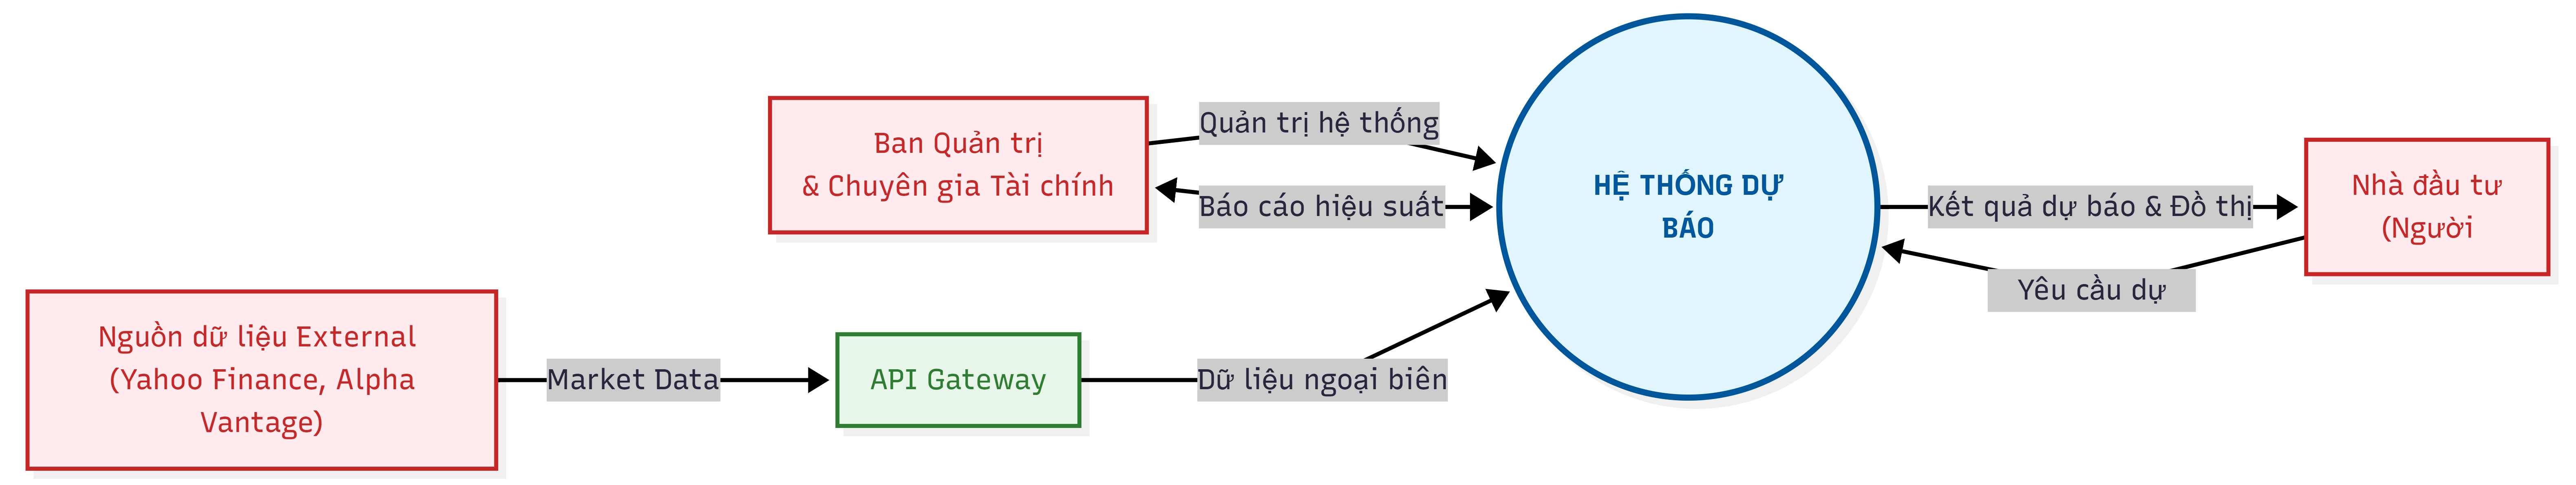
\includegraphics[width=1\textwidth]{images/context-diagram.png}
          \end{figure}

          \newpage

          \begin{itemize}
              \item System boundaries and external entities (Level 0)
          \end{itemize}

          \begin{figure}[htbp]
              \centering
              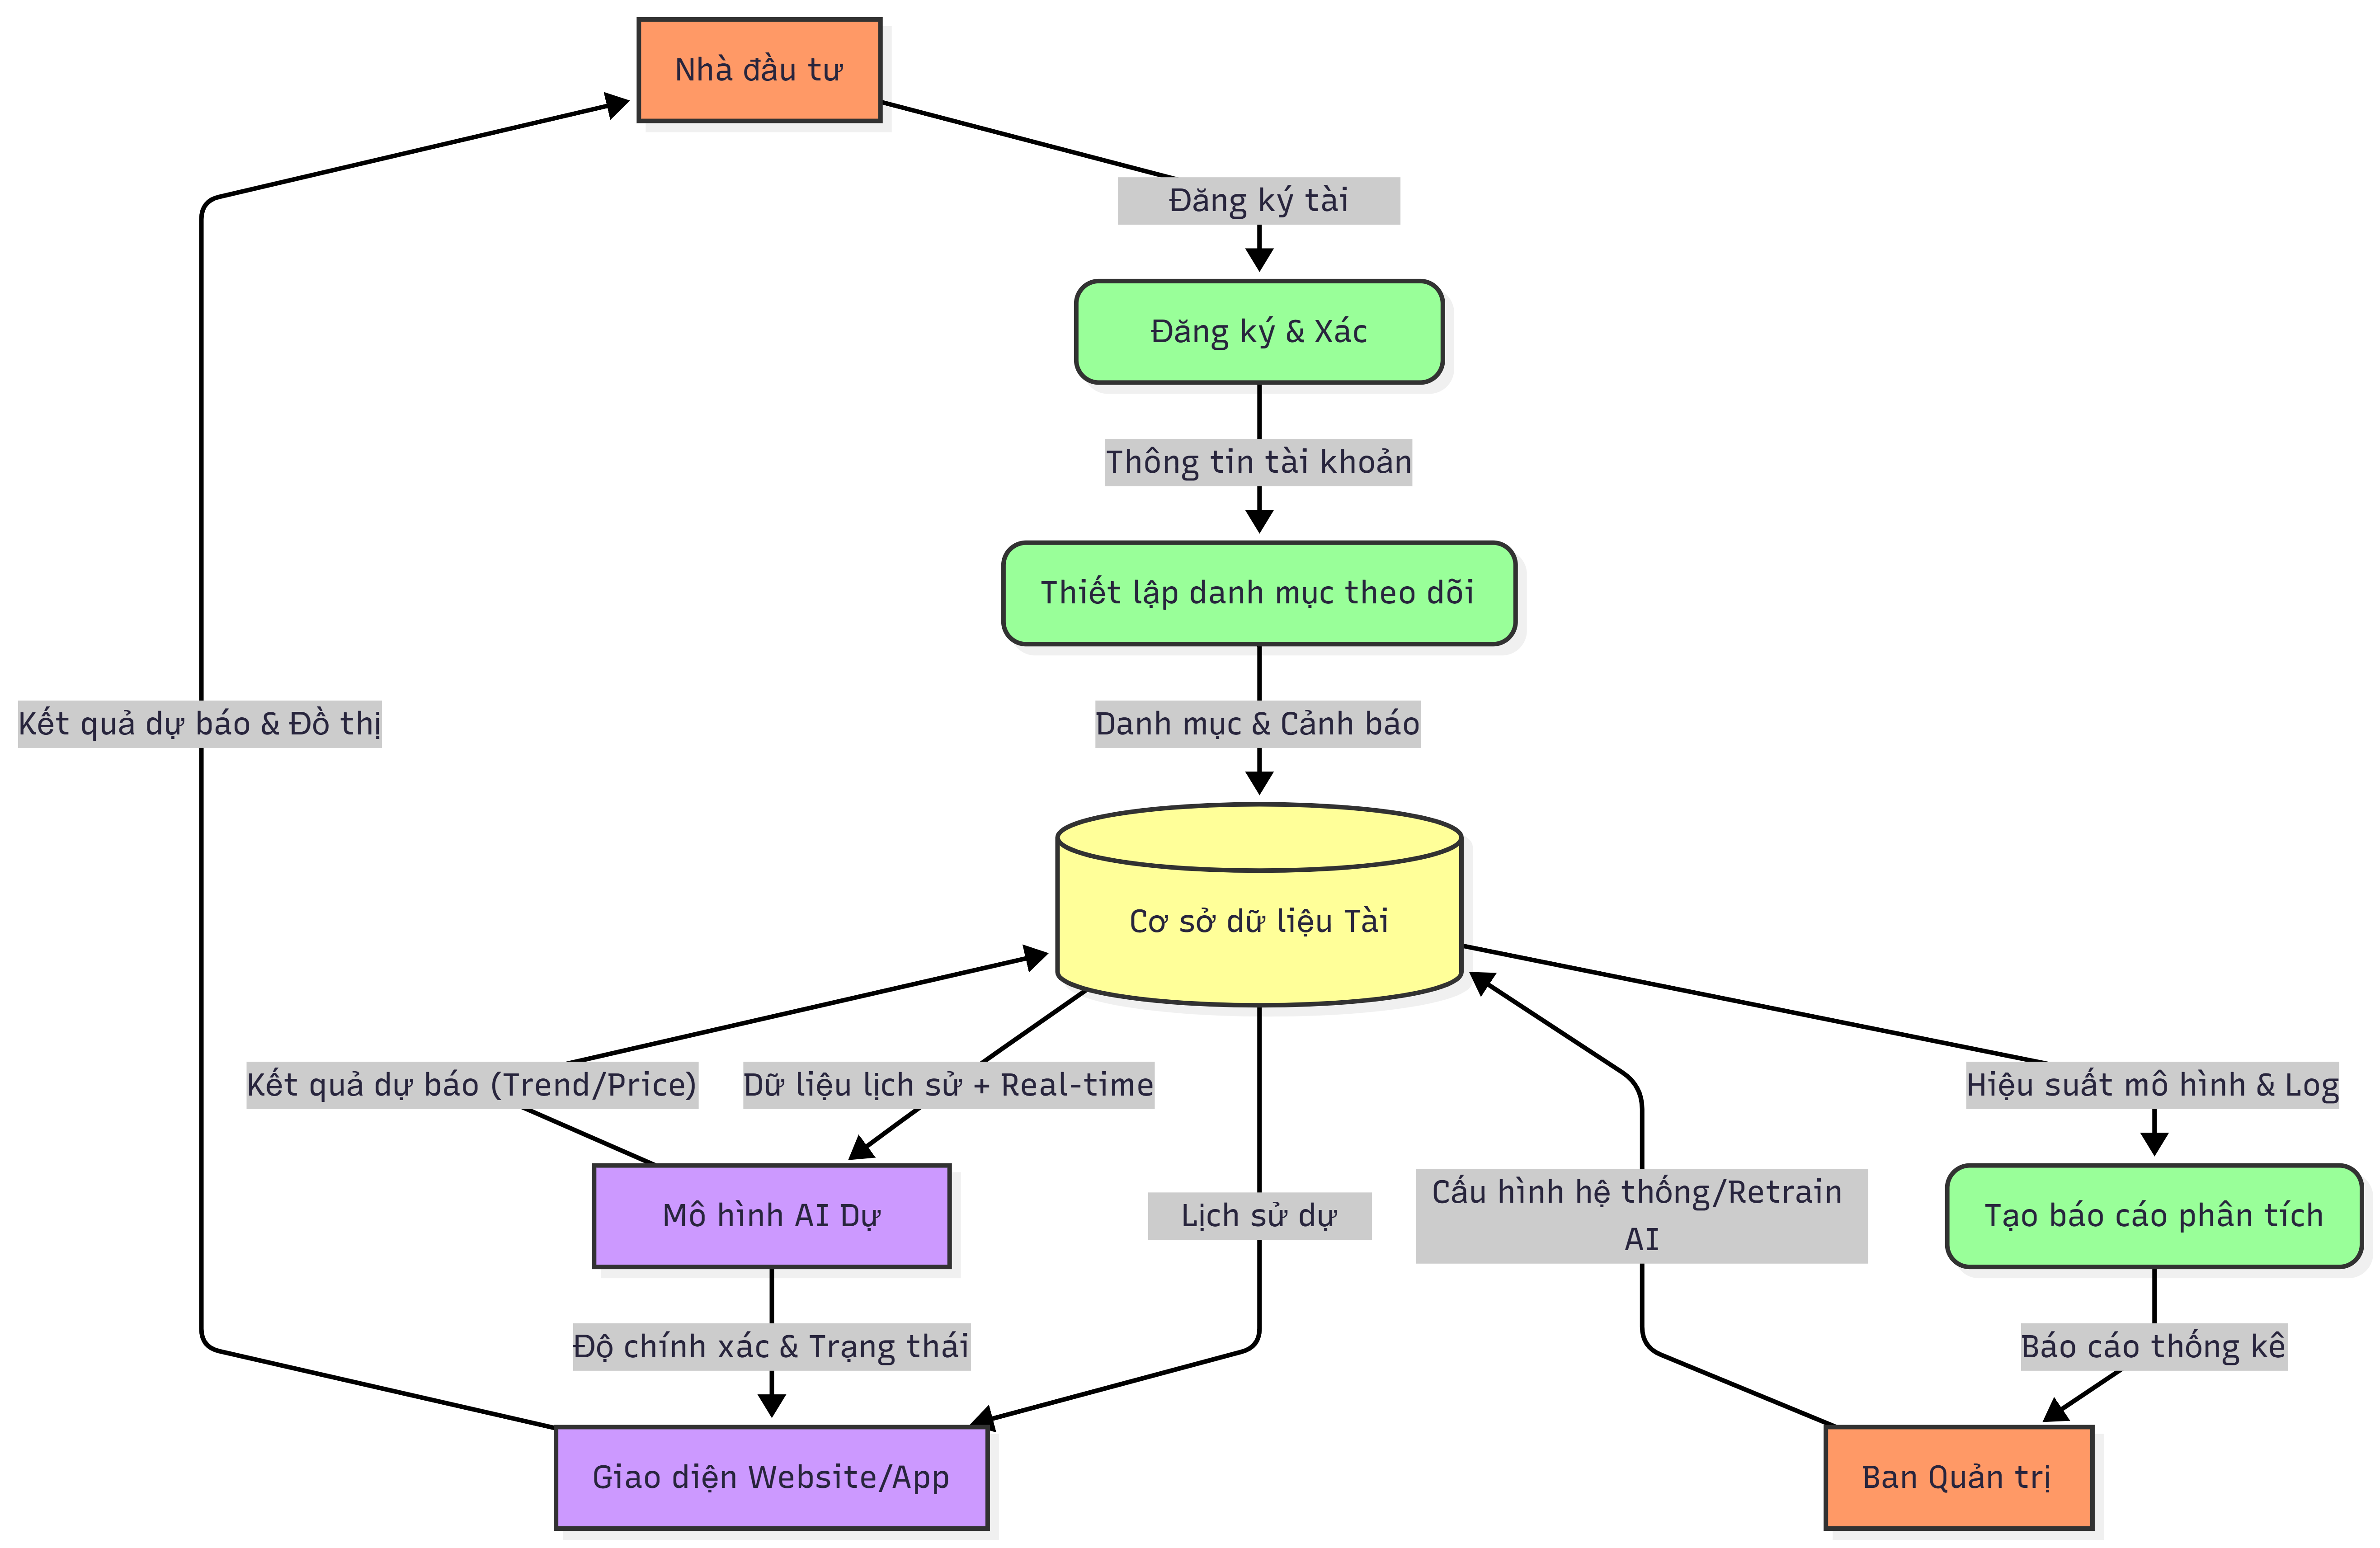
\includegraphics[width=1\textwidth]{images/data-flow.png}
          \end{figure}

          \newpage

    \item \textbf{AI Engine Component Diagram }
          \begin{figure}[htbp]
              \centering
              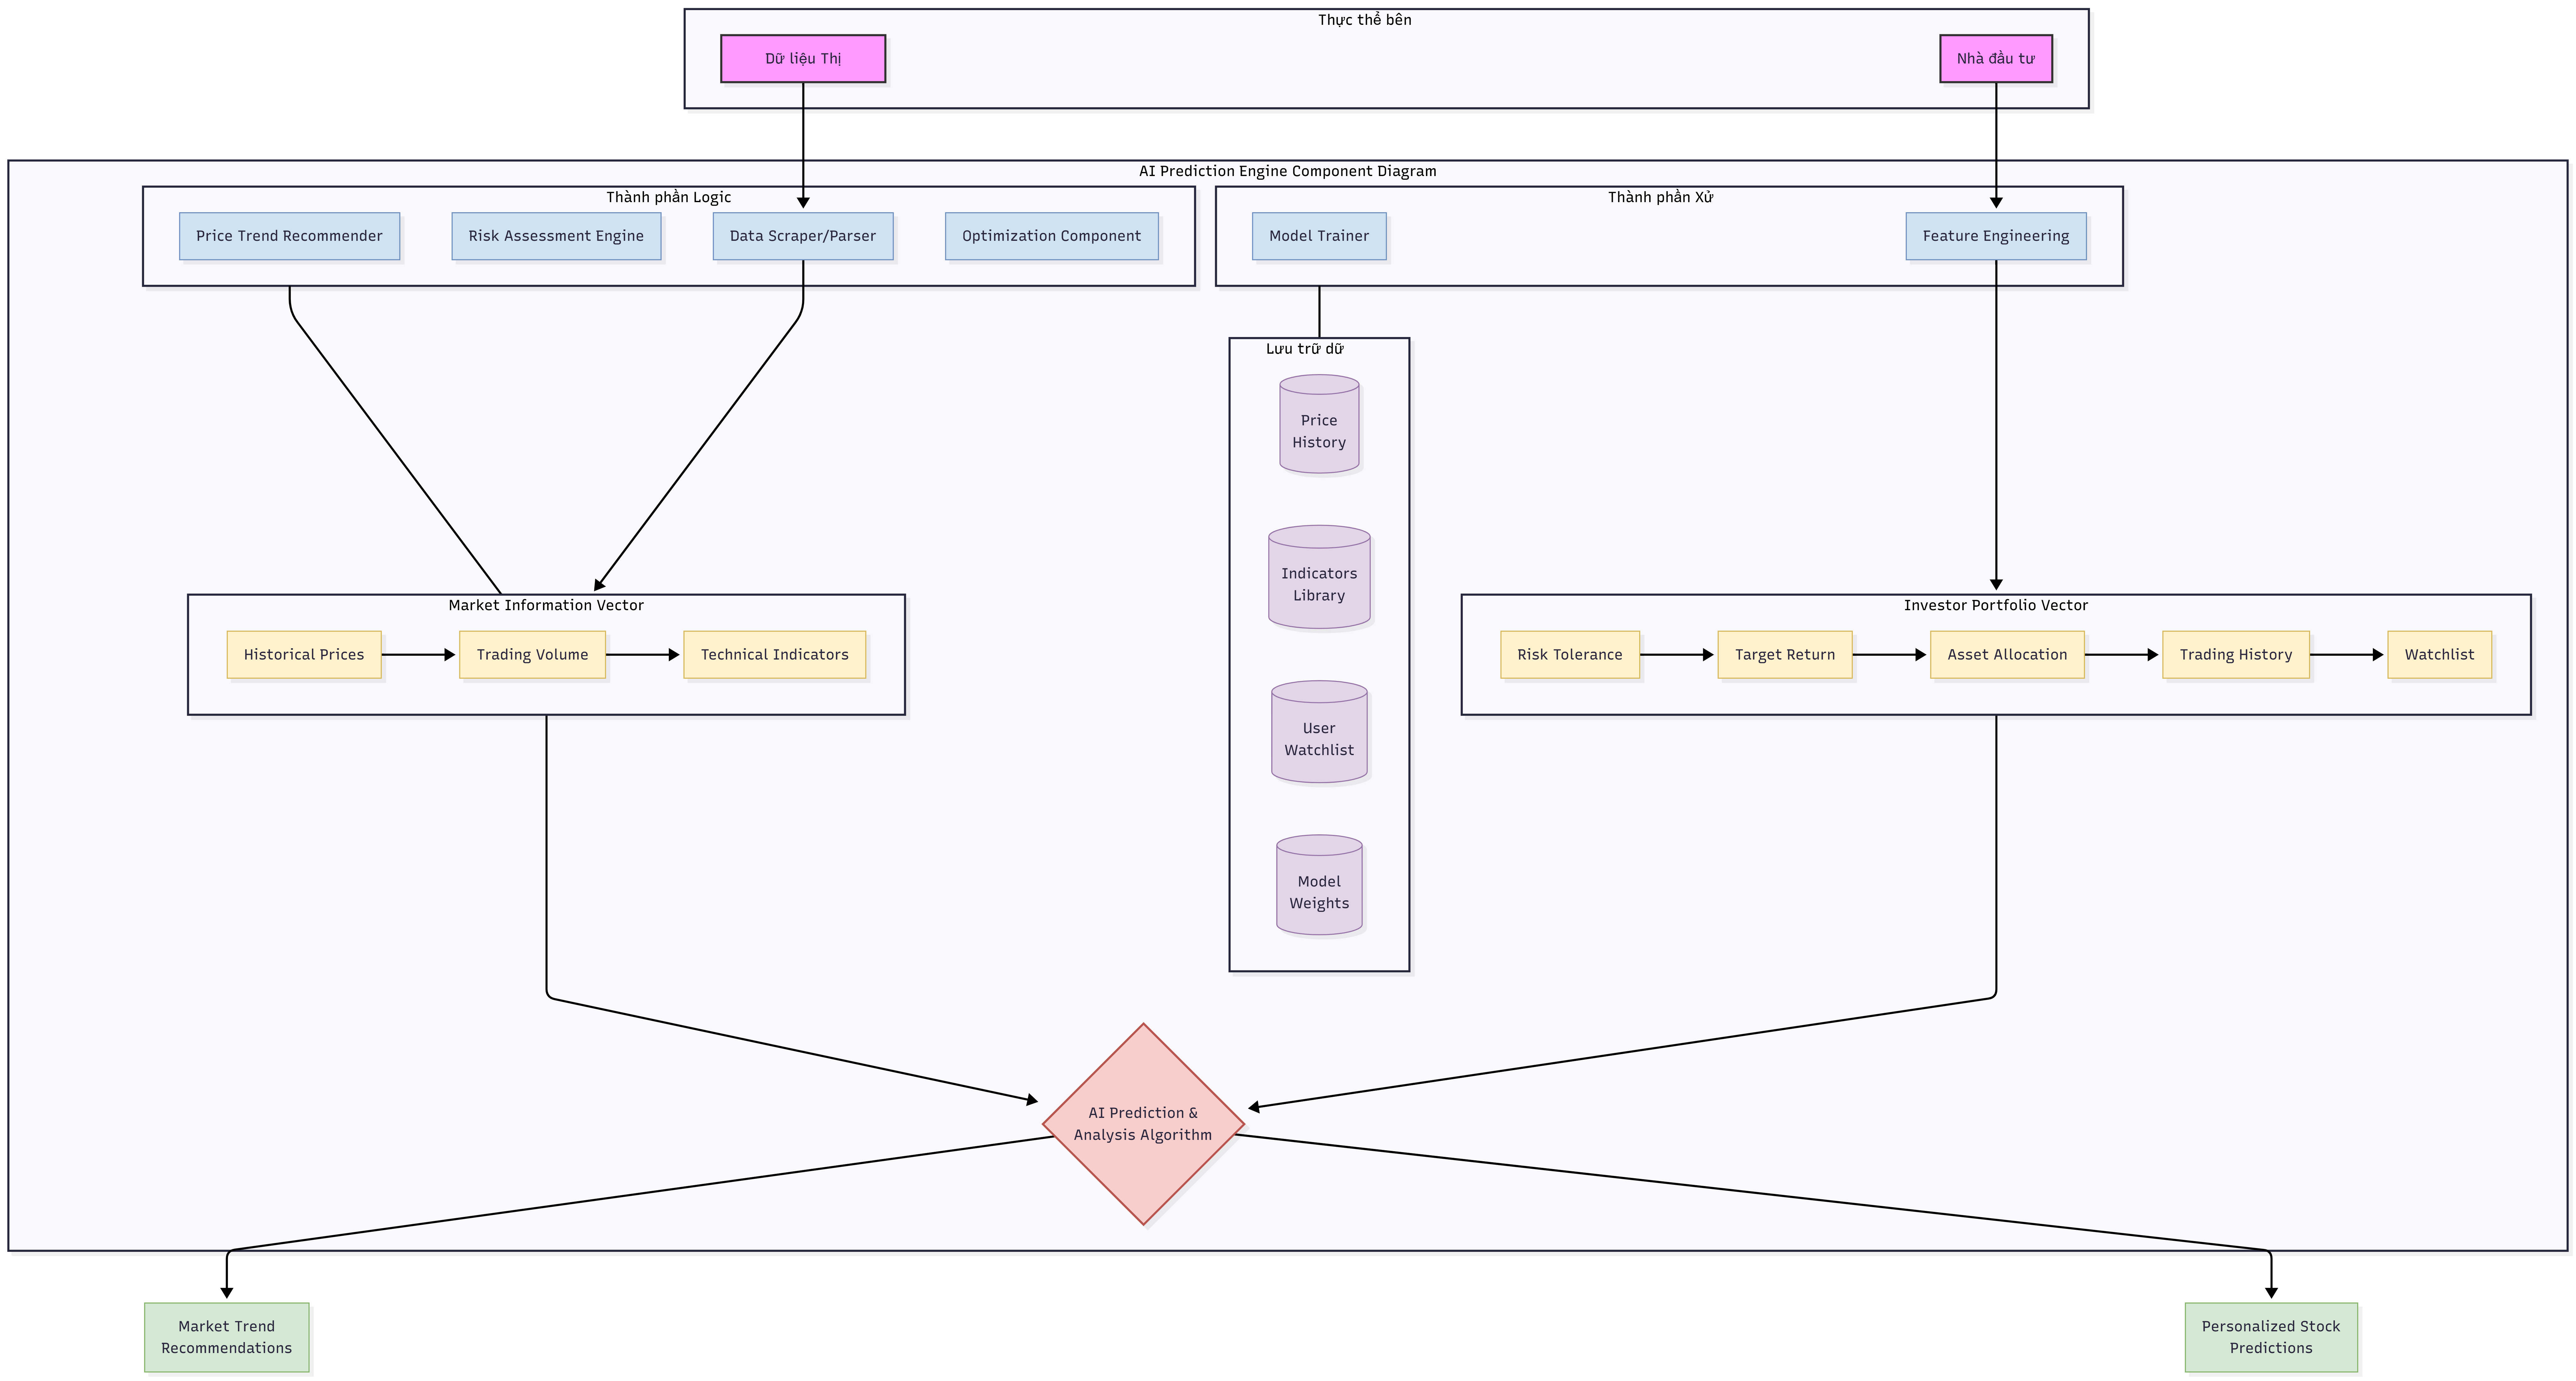
\includegraphics[width=1\textwidth]{images/AI-engine-component-diagram.png}
          \end{figure}

    \item \textbf{Process Flow Diagrams}
          \begin{itemize}
              \item Dữ liệu chứng khoán và quá trình xử lý của ứng dụng
          \end{itemize}
          \begin{figure}[htbp]
              \centering
              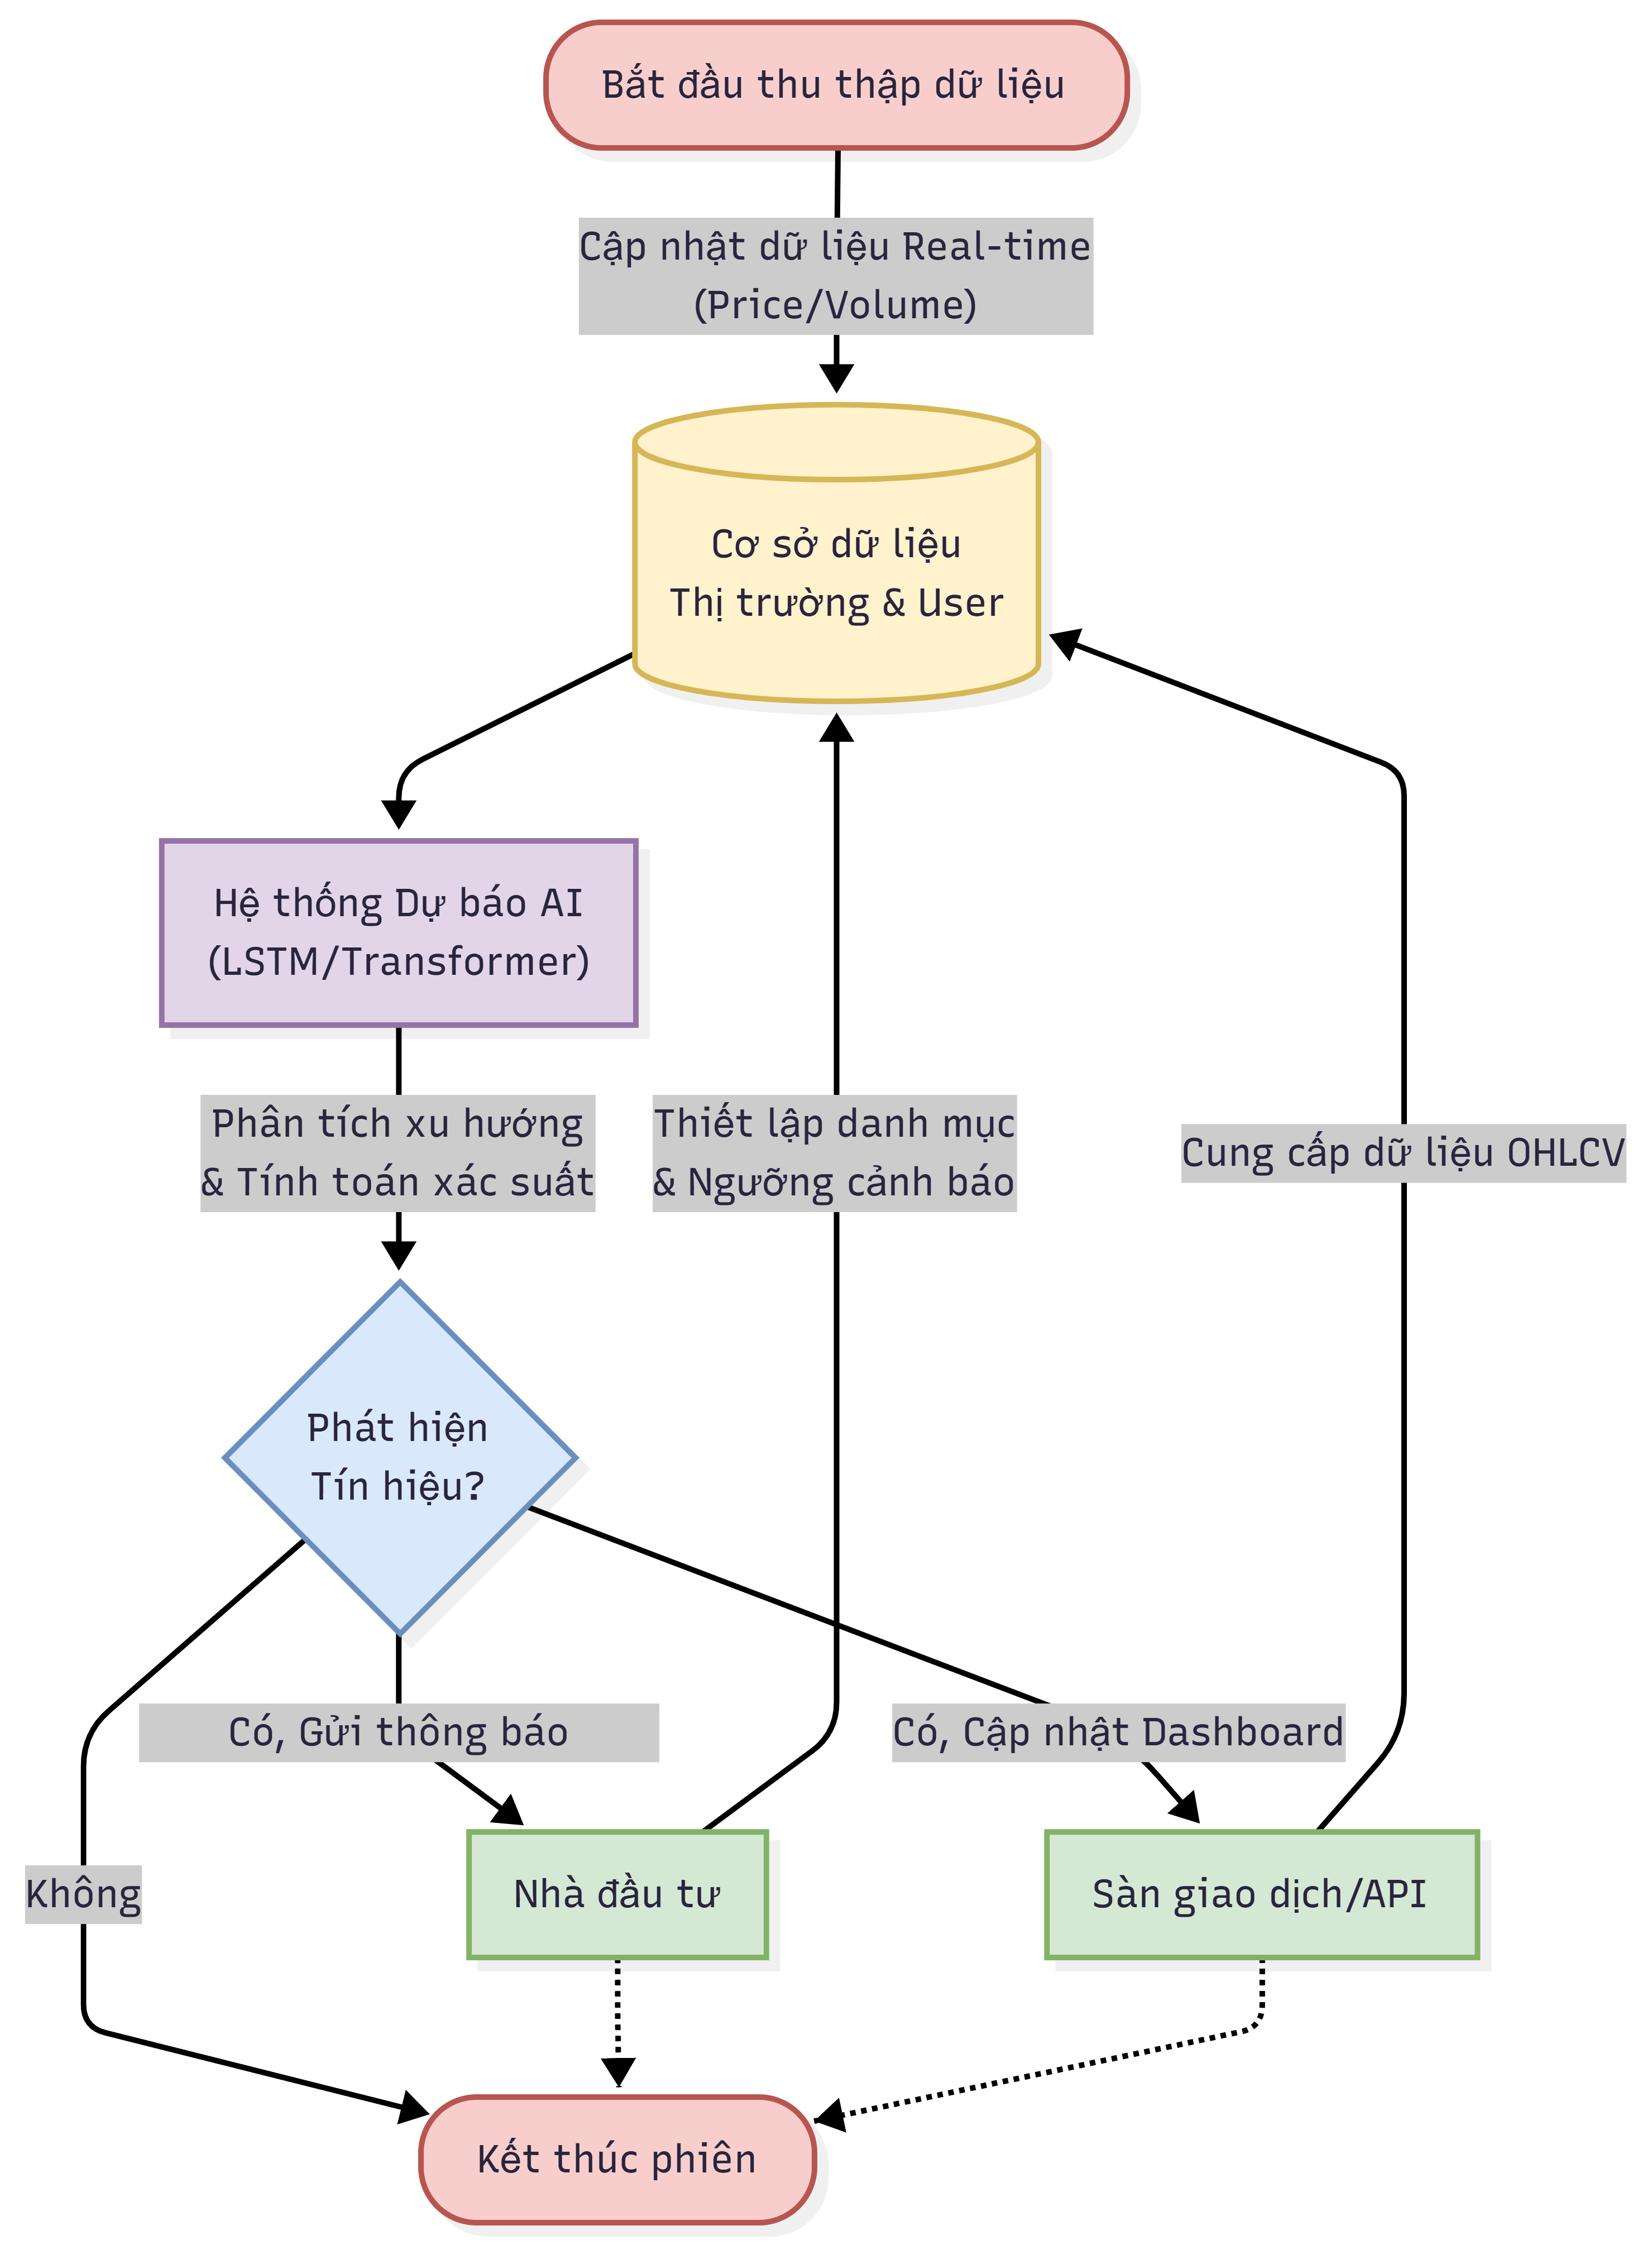
\includegraphics[width=1\textwidth]{images/process-flow.png}
          \end{figure}

          \newpage

          \begin{itemize}
              \item Người dùng đăng kí và quản lý danh mục
          \end{itemize}
          \begin{figure}[htbp]
              \centering
              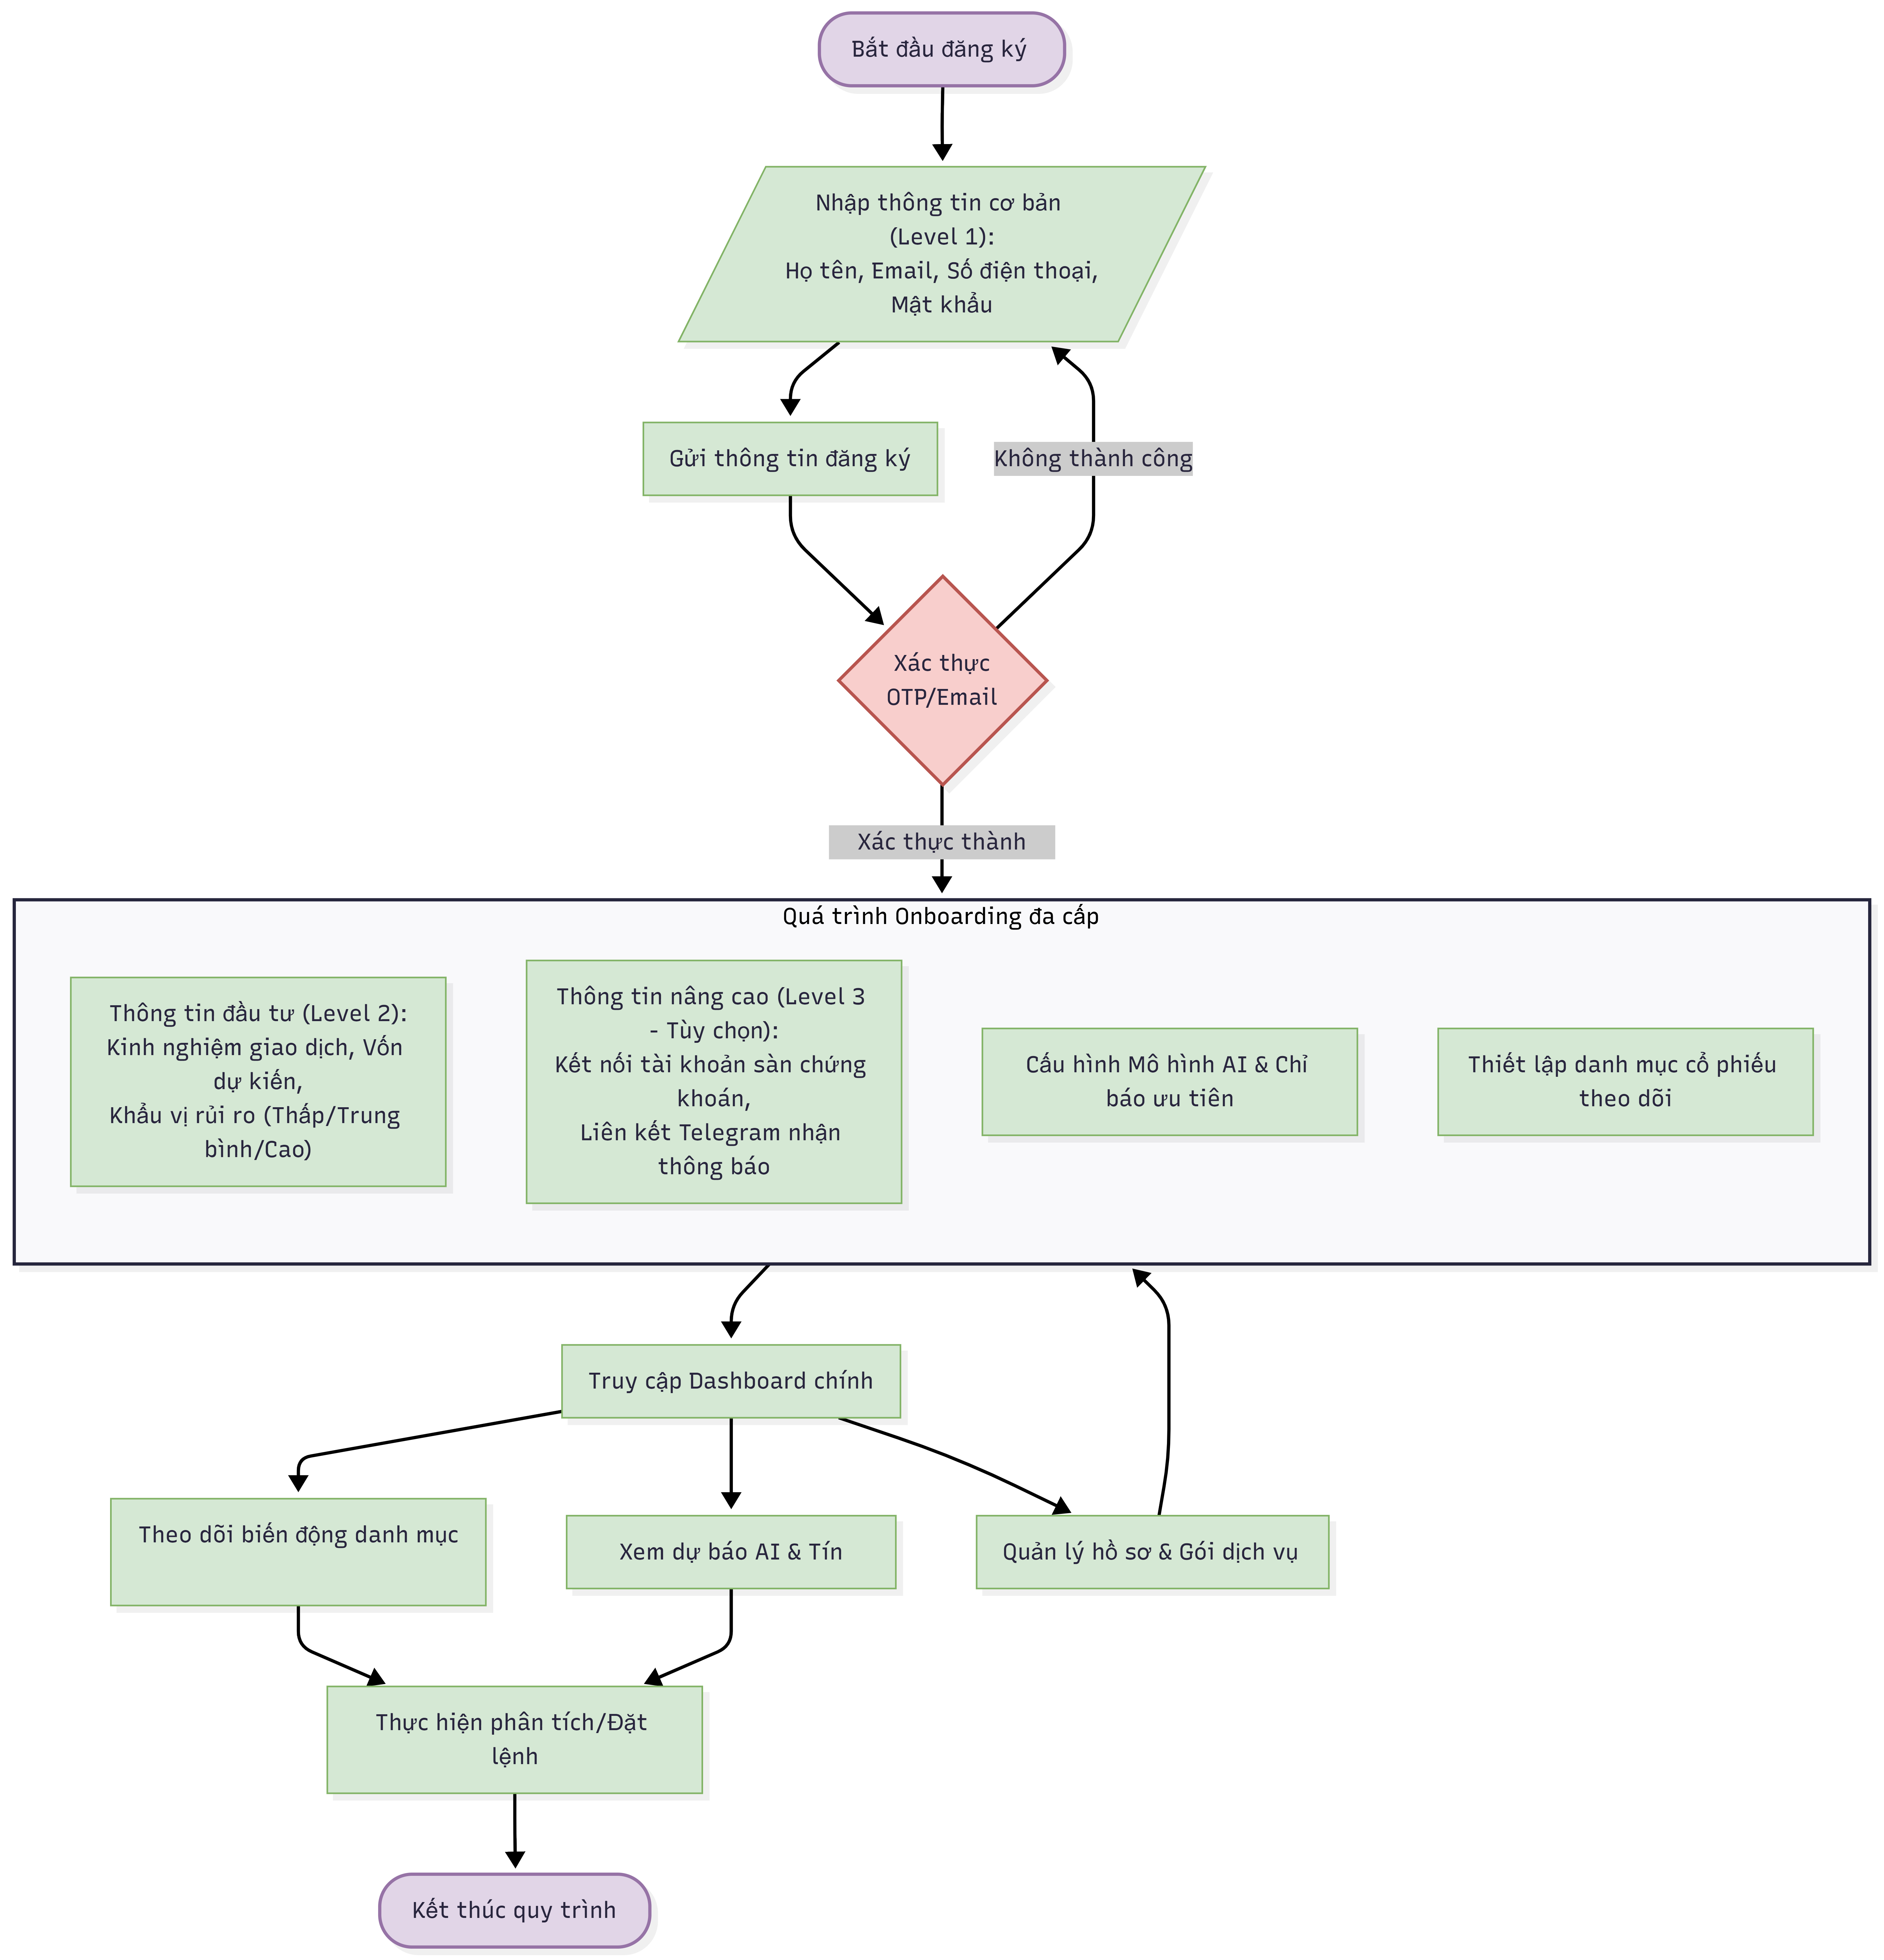
\includegraphics[width=1\textwidth]{images/registration-flow.png}
          \end{figure}

          \begin{itemize}
              \item Biểu đồ Use Case Nhà đầu tư
          \end{itemize}
          \begin{figure}[H]
              \centering
              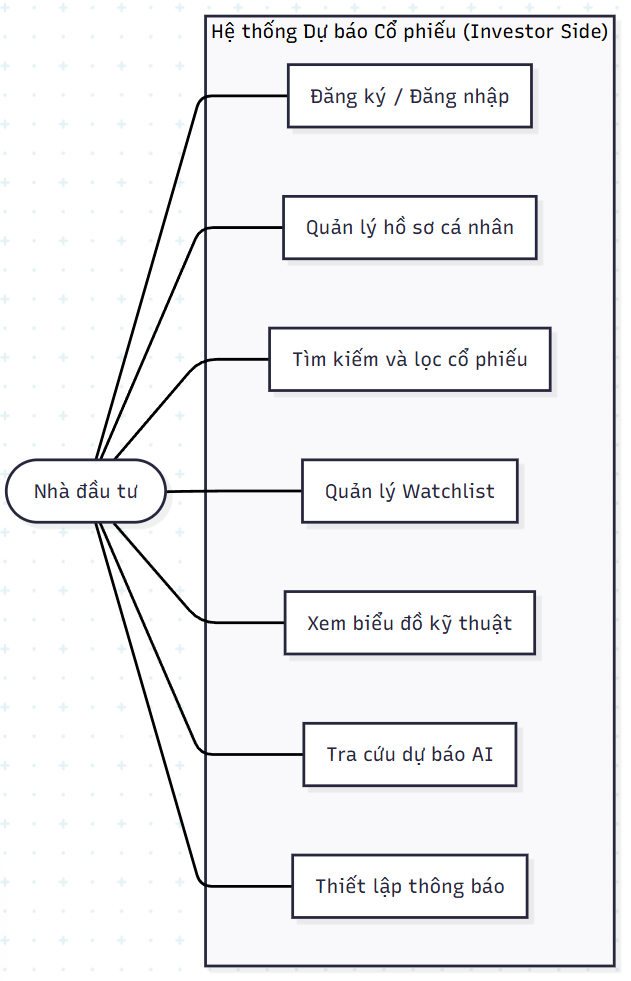
\includegraphics[width=0.9\textwidth]{images/investor-use-case.png}
          \end{figure}
          \newpage

          \begin{itemize}
              \item Biểu đồ Use Case Quản trị viên
          \end{itemize}
          \begin{figure}[htbp]
              \centering
              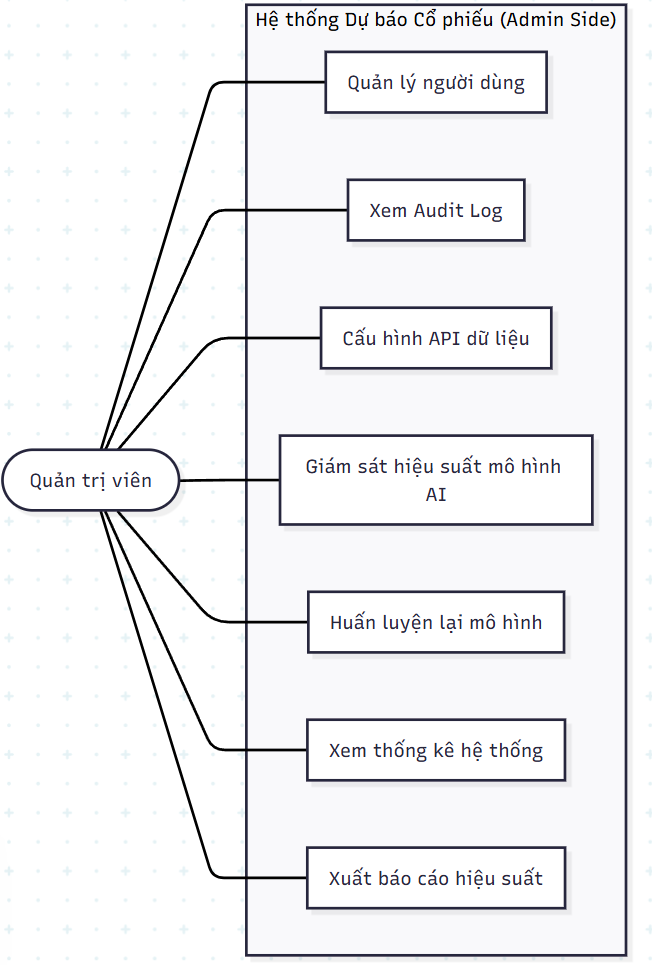
\includegraphics[width=0.9\textwidth]{images/admin-use-case.png}
          \end{figure}

          \begin{itemize}
              \item Database
          \end{itemize}
          \begin{landscape}
          \begin{figure}[H]
              \centering
              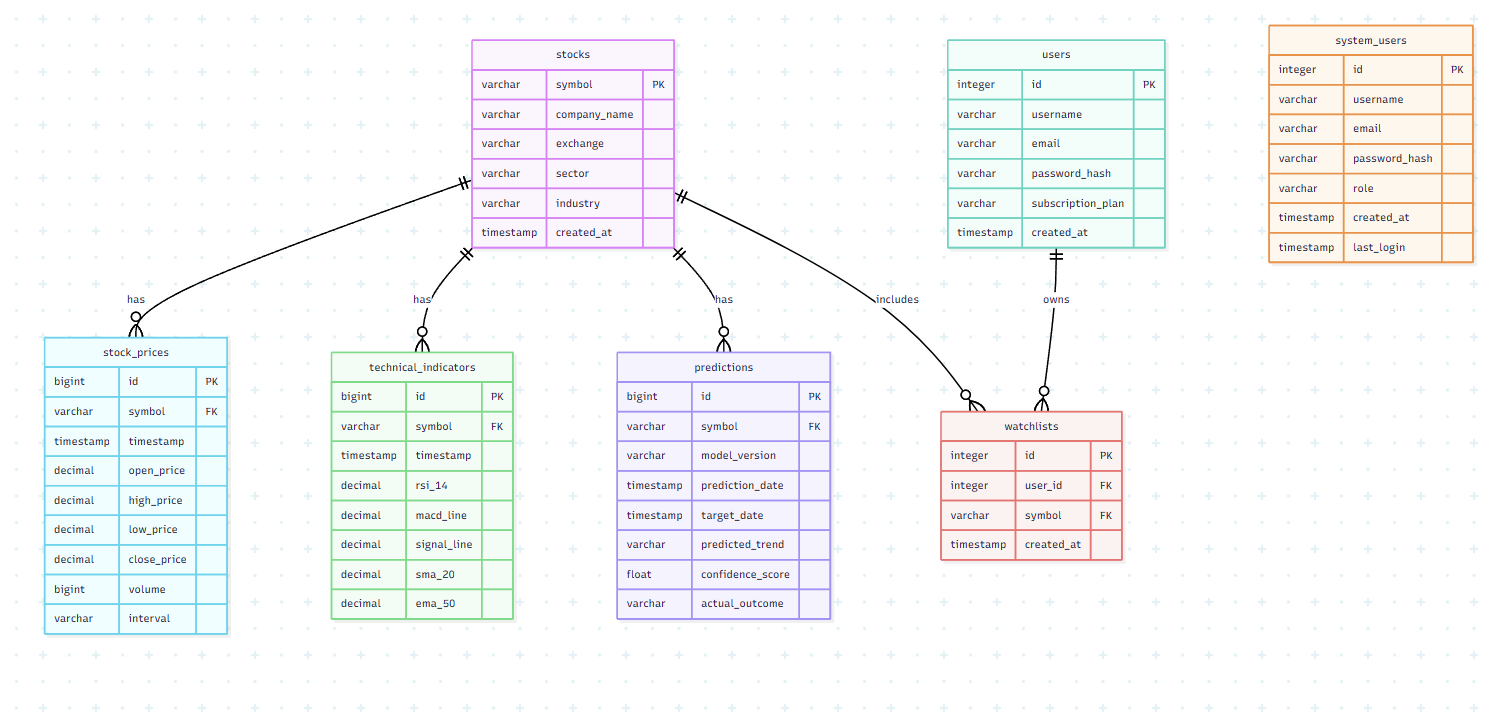
\includegraphics[width=1\linewidth]{images/database.png}
          \end{figure}
          \end{landscape}
          \clearpage

          \begin{itemize}
              \item Luồng điều hướng giao diện người dùng (UI Flow)
          \end{itemize}
          \begin{figure}[H]
              \centering
              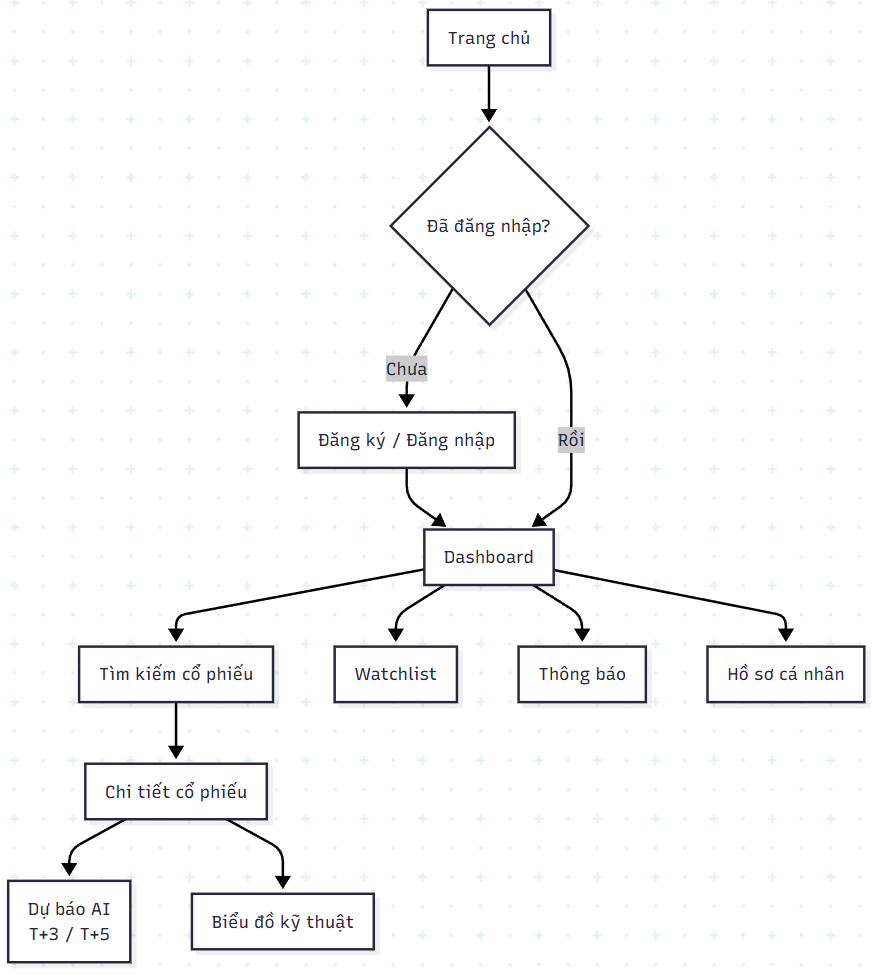
\includegraphics[width=0.85\textwidth]{images/ui-flow.png}
          \end{figure}

\end{enumerate}

\section{Phụ lục B: Danh sách các vấn đề cần giải quyết (Issues List)}

Phụ lục này ghi nhận các vấn đề còn tồn đọng và các câu hỏi chưa được giải quyết trong quá trình phát triển hệ thống \textit{Website dự đoán giá cổ phiếu ngắn hạn}. Các nội dung này cần được làm rõ trong các giai đoạn tiếp theo của dự án.

\subsection{Tích hợp nguồn dữ liệu (Data Integration)}
\begin{itemize}
    \item Xác định chi tiết các nguồn dữ liệu thị trường chứng khoán sẽ được tích hợp, bao gồm API giá cổ phiếu, dữ liệu lịch sử giao dịch và dữ liệu thời gian thực.
    \item Cung cấp tài liệu API, cơ chế xác thực truy cập và giới hạn sử dụng từ các nhà cung cấp dữ liệu.
\end{itemize}

\subsection{Kiến trúc triển khai hệ thống (Deployment Architecture)}
\begin{itemize}
    \item Lựa chọn phương án triển khai hệ thống: Cloud, On-premises hoặc kiến trúc lai (Hybrid).
    \item Xác định yêu cầu về hạ tầng, khả năng mở rộng hệ thống và hiệu năng xử lý dữ liệu theo thời gian thực.
\end{itemize}

\subsection{Thu thập và xử lý dữ liệu (Data Collection \& Processing)}
\begin{itemize}
    \item Thống kê và mô tả chi tiết tập dữ liệu lịch sử và dữ liệu thời gian thực phục vụ mô hình dự đoán.
    \item Xây dựng phương pháp làm sạch dữ liệu, chuẩn hóa và tiền xử lý dữ liệu chuỗi thời gian nhằm đảm bảo chất lượng đầu vào cho mô hình.
\end{itemize}

\subsection{Lựa chọn mô hình học máy (Machine Learning Model Selection)}
\begin{itemize}
    \item Xác định các thuật toán dự đoán phù hợp cho bài toán dự báo giá cổ phiếu ngắn hạn (ví dụ: ARIMA, LSTM hoặc mô hình kết hợp).
    \item Xác định yêu cầu về dữ liệu huấn luyện, phương pháp trích chọn đặc trưng (feature engineering) và nguồn dữ liệu sử dụng để huấn luyện mô hình.
\end{itemize}

\vspace{0.5cm}
\noindent\textit{Ghi chú: Danh sách này sẽ được cập nhật và mở rộng trong suốt vòng đời phát triển của dự án.}

\end{document}